%\documentclass[pdftex,nosumlimits,final,compress,english]{beamer}
\documentclass[pdftex,final,compress,english]{beamer}
% \documentclass[pdftex,nosumlimits,final,compress, handout,norsk]{beamer}

\usetheme[norsk]{UiO}

\usepackage[latin1]{inputenc}
\usepackage[english]{babel}
\usepackage{times}
\usepackage[T1]{fontenc}
\usepackage{calc}
\usepackage{amsmath}

 \mode<handout>{
% \mode<all>{
\usepackage{pgfpages}
\pgfpagesuselayout{4 on 1}[a4paper,landscape,border shrink=2mm]
% \pgfpagesuselayout{8 on 1}[a4paper,border shrink=5mm]
% \setbeamercolor{background canvas}{bg=black!5}
 }


% If you wish to uncover everything in a step-wise fashion, uncomment
% the following command: 

%\beamerdefaultoverlayspecification{<+->}


% Use some nice templates

% \beamertemplateshadingbackground{red!10}{structure!10}
% \beamertemplatetransparentcovereddynamic
% \beamertemplateballitem
% \beamertemplatenumberedballsectiontoc


%
% Some definitions:
%
\definecolor{LightSkyBlue}{RGB}{135,206,250}
\setbeamercolor{lowcol}{fg=black,bg=LightSkyBlue!90!black}
%\setbeamercolor{lowcol}{fg=black,bg=cyan!10!black}

\newlength{\bredde}
\newcommand{\FigBox}[1]{% #1=Image,
  \setlength{\bredde}{\widthof{#1}}
  %\centerline{
    \begin{beamerboxesrounded}[width=\bredde,lower=lowcol,shadow=true]{}
      \centering 
      #1%
    \end{beamerboxesrounded}
  %}%
}

\newcommand{\bm}[1]{\mbox{\boldmath{$#1$}}}


\title[]{\bf\LARGE{\textcolor{black}
{ADAPTIVE BEAMFORMING IN\\ ACTIVE SONAR IMAGING}}}
\author[]{Andreas~Austeng$^{\text{a}}$, Are~F~C~Jensen$^{\text{a}}$, Safiye~Jetlund$^{\text{}}$, Roy~E~Hansen$^{\text{a,b}}$ and Sverre~Holm$^{\text{a}}$}
\date[Andreas Austeng at Geilo, Feb.\ 2010]{Geilo, February 2010}
\institute[Dept.\ of Informatics, University of Oslo]{\bf$^{\text{a}}$Department of Informatics, University
  of Oslo\\
$^{\text{b}}$Norwegian Defence Research Establishment, Kjeller}


\begin{document}

%% Draft-mode!
% \usebackgroundtemplate{
%   \includegraphics[width=\paperwidth,
%                    height=\paperheight]{Draft}
% }


\begin{frame}
\vspace*{2\baselineskip}
  \titlepage
\end{frame}
\note{\null{}}

\section<presentation>*{Outline}

\begin{frame}
  \frametitle{Outline of this talk}
  \tableofcontents[part=1]% ,hideallsubsections]
\end{frame}


%\AtBeginSection[]
%{
%  \begin{frame}% <beamer,handout>
%    \frametitle{Outline}
%    %    \tableofcontents[current,currentsection]
%    \tableofcontents[sectionstyle=show/hide,subsectionstyle=show/show/hide]
%  \end{frame}
%}


%%%%%%%%%%%%%%%%%%%%%%%%%%%%%%%%%%%%%%%%%%%%%%%%%%%%%%%%%%%%
%% Start p� 'innmat' forelesning 
%%
%%%%%%%%%%%%%%%%%%%%%%%%%%%%%%%%%%%%%%%%%%%%%%%%%%%%%%%%%%%%

\part{}

 \section[]{Beamforming}
\subsection[]{Conventional beamforming}
\frame{
  \frametitle{Beamforming;\\ focus and steering of beams}
  \hspace*{.1\textwidth}{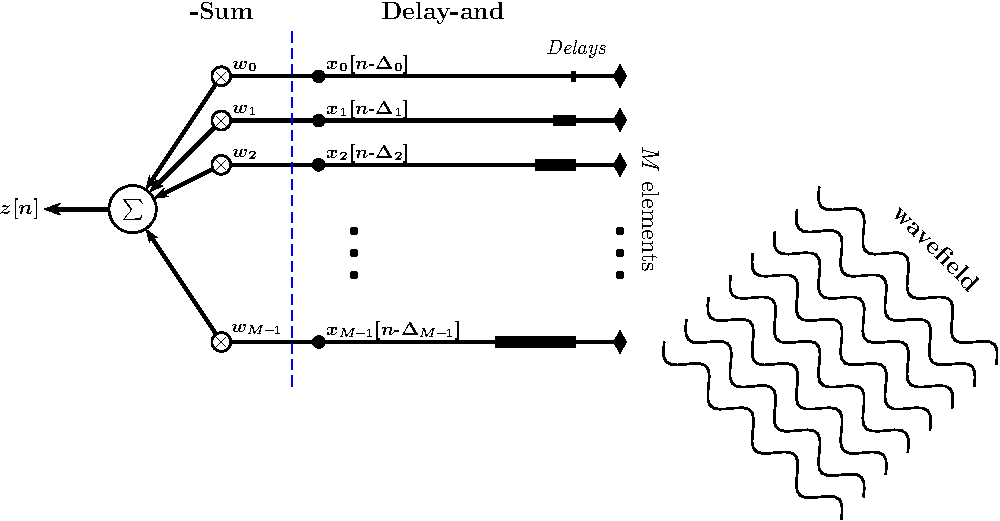
\includegraphics[width=.9\textwidth]{Figs/das}}
  
  \vspace*{-2.2\baselineskip}
  %\indent
    
  \vspace*{.5\baselineskip}
  \FigBox{$z[n] = \sum_{m=0}^{M-1}\ w_m^*[n]\ x_m[n-\Delta_m] =
    \bm{w}^H[n] \bm{X}[n]$}

 \FigBox{%
   \vbox{\small
     \hbox{Receiving signal:}%\\
     \hbox{$\bm{X}[n] = A[n]\ \bm{a}(\bm{k_0}) + \bm{S}[n]$,}%\\
     \hbox{$A[n]$; ampl. of signal in direction $\bm{k_0}$, and $\bm{S}[n]$; noise.}
   }%}
  }
}

 
%\section[]{}
%\subsection[]{}
\frame{
  %\frametitle{DAS weighting}
  \begin{columns}
    \begin{column}{.35\textwidth}
      \noindent\FigBox{\parbox{\textwidth}{\small%
          Conventional beam\-formers uses pre-defined sensor weights}}
    \end{column}
    \begin{column}{.5\textwidth}
      \vspace*{2\baselineskip}
      
      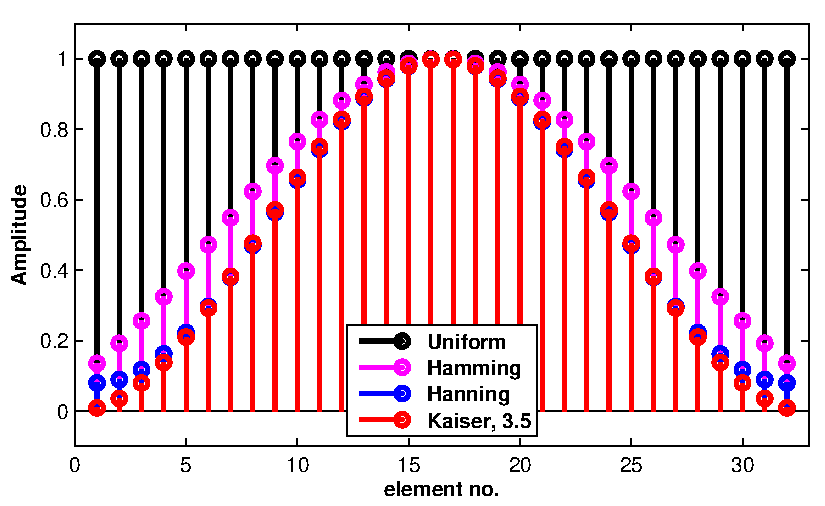
\includegraphics[width=.95\textwidth]{Figs/VindusFunk}\newline
      % \hspace*{.35\textwidth}
      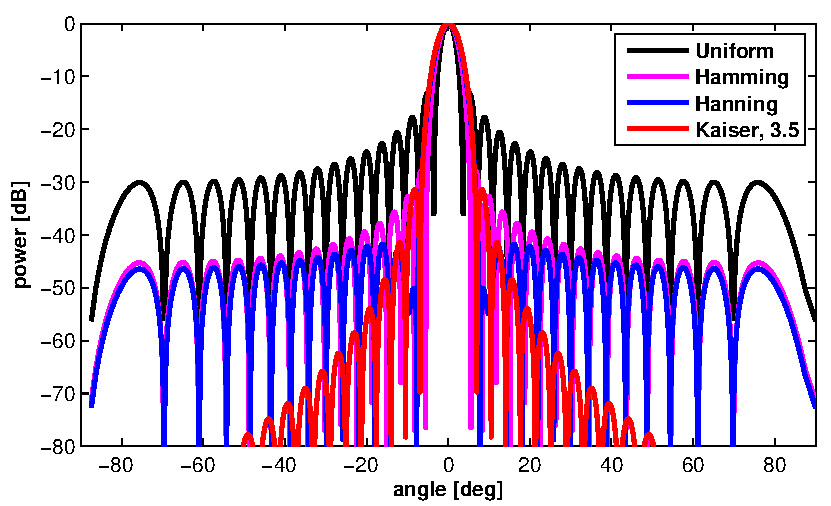
\includegraphics[width=.95\textwidth]{Figs/RespVindusFunk}
    \end{column}
  \end{columns}
  
  % \vspace*{.1\textheight}
  \FigBox{\parbox{.9\textwidth}{\small%
      Adaptive beam\-formers uses the statistics of the data to
      estimates weights for each direction and each range}}      
  \vspace*{\baselineskip}
}

%\section[]{}
\subsection[]{Adaptive beamforming, MV and APES}
\frame{
  \frametitle{Minimum Variance (MV) beamformer}
  \begin{itemize}
  \item Known by several names
    \begin{itemize}
    \item Minimum Variance Distortionless Response (MVDR) beamformer
    \item Capon method or Capon beamformer
    \item (Apes beamformer)
    \end{itemize}
  \item Problem to solve:
    \begin{itemize}
    \item Find the weights that minimize the variance (power) of z[n] (the
      beamformer output) with the constraint that the signal that
      originates from the steering direction is passed with unity gain
    \end{itemize}
  \end{itemize}
}


%\section[]{}
%\subsection[]{}
\frame{
%  \frametitle{}
  \noindent\textbf{\large MV BF passes the signal of interest with
    unity gain while an interferring signal is suppressed}
  \newline
  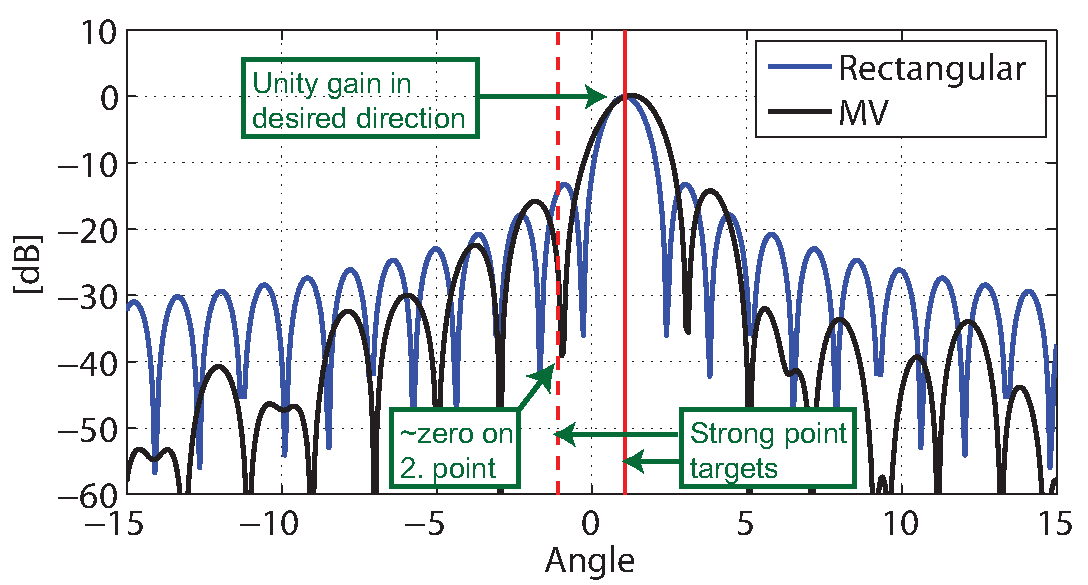
\includegraphics[width=.9\textwidth]{Figs/BeampatternPoints}
}

\frame{
%  \frametitle{}
  \noindent\textbf{\large MV BF allowes large sidelobes in regions
    with low energy}  
  \newline
  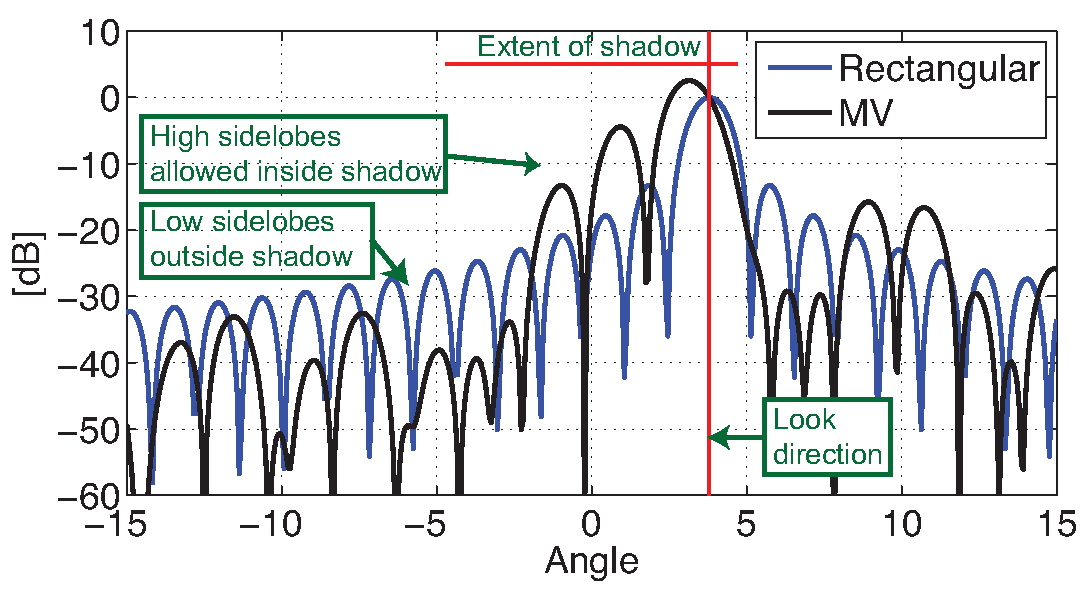
\includegraphics[width=.9\textwidth]{Figs/BeampatternCyst}
}


%\section[]{}
%\subsection[]{}
\frame{
  \frametitle{Minimum Variance (MV) beamformer}
  \begin{itemize}
  \item Variance: $E\{|z[n]|^2\} = E\{|\bm{w}^H\bm{X}[n]|^2\} = \bm{w}^H\bm{R w}$, where $\bm{R}=E\{\bm{XX}^H\}$ is the spatial covariance matrix.
  \end{itemize}
  \noindent\FigBox{\parbox{\textwidth}{%\small%
      Problem formulation:
      \begin{eqnarray*}        
        \bm{w}_{mvdr}&=& \min_{\bm{w}}\ \bm{w}^H\bm{R w}
        =\min_{\bm{w}}\ \bm{w}^H\left(|A|^2 \bm{a}(\bm{k_0})\bm{a}(\bm{k_0})^H + \bm{R}_S\right) \bm{w} \\
        &=& \min_{\bm{w}}\bm{w}^H \bm{R}_S \bm{w}\\
        \text{s.t.} &&\bm{w}^H \bm{a}(\bm{k_0})=1
      \end{eqnarray*}
      Solution:\\
      $\bm{w}_{mvdr} = \frac{\bm{R}^{-1} \bm{a}(\bm{k_0})}%
      {\bm{a}(\bm{k_0})^H \bm{R}^{-1} \bm{a}(\bm{k_0})} = %
      \frac{\bm{R}_S^{-1} \bm{a}(\bm{k_0})}%
           {\bm{a}(\bm{k_0})^H \bm{R}_S^{-1} \bm{a}(\bm{k_0})}$
    }
  }
}


%\section[]{}
%\subsection[]{}
\frame{
  \frametitle{MV: Known problems and solutions}
%
  \begin{tabular}{lcl}
    \textbf{\large Known problems} &
    & % \textcolor{blue}{$\bm{\Longrightarrow}$} &
    \textbf{\large Solutions} \\
%
    \parbox[t]{.38\textwidth}{
      Robustness
      \begin{itemize}
      \item with respect to steering vector and gain differences
        across the array
      \end{itemize}} &
    \textcolor{blue}{$\bm{\Longrightarrow}$} &
    \parbox[t]{.4\textwidth}{
      Diagonal loading
      \begin{itemize}
      \item Estimate $\bm{R}$ as $\bm{\tilde{R}} = \bm{\hat{R}} +
        \epsilon \bm{I}$
      \end{itemize}
    }\\
    & & \\
    & & \\
    & & \\
    & &
    \rlap{\hspace*{-.3cm}\raisebox{0cm}[0pt][0pt]{\mbox{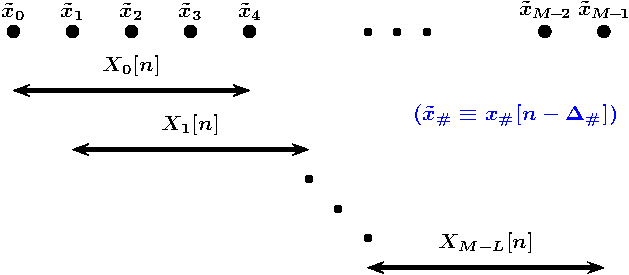
\includegraphics[width=
            .5\textwidth]{Figs/subarray}}}}
 \\
%
    \parbox[t]{.38\textwidth}{
      Signal cancellation
      \begin{itemize}
      \item cancellation of coherent signals 
      \end{itemize}} &
    \textcolor{blue}{$\bm{\Longrightarrow}$} &
    \parbox[t]{.4\textwidth}{
      Sub-array averaging
      \begin{itemize}
      \item Estimate $\bm{R}$ by spatial averaging
      \end{itemize}
    }

  \end{tabular}
}




%\section[]{}
%\subsection[]{}
\frame{
  \frametitle{MV (Capon) vs.\ Apes beamformer}
  \begin{itemize}
  \item MV (Capon):
    \begin{itemize}
    \item Minimize the spatial covariance matrix $\bm{R}$.
    \item High angular resolution.
    \item Known to have problems with signal cancellation and robustness.
    \item Sensitive to choice of parameters.
    \end{itemize}
  \item Apes:
    \begin{itemize}
    \item Minimize the ``interference and noise covariance matrix'' $\bm{R}_s$.
    \item Better amplitude estimates than MV.
    \item Does not offer quite the same resolution as the MV beamformer.
    \end{itemize}
  \end{itemize}
}


%\section[]{}
\subsection[]{Beamspace processing}
\frame{
  \frametitle{Beamspace processing}
  \begin{itemize}
  \item MV/Apes: Must find $\bm{R}^{-1}$. 
    \begin{itemize}
    \item 32-els array, size of $\bm{R}$: 12$\times$12
      to  16$\times$16.
    \item Complexity: $o(12^3)=o(1728)$ to $o(16^3)=o(4096)$.
    \end{itemize}
  \item Possibly to project our data into a subspace described by
    ortogonal beams; Beamspace.
    \begin{itemize}
    \item By using 4 beams, the complexity reduces to $o(4^3) =
      o(64)$, 
    \item 64/4096 = 1/64  !!!
    \end{itemize}
  \item Should be possible to do in real time!
  \end{itemize}
  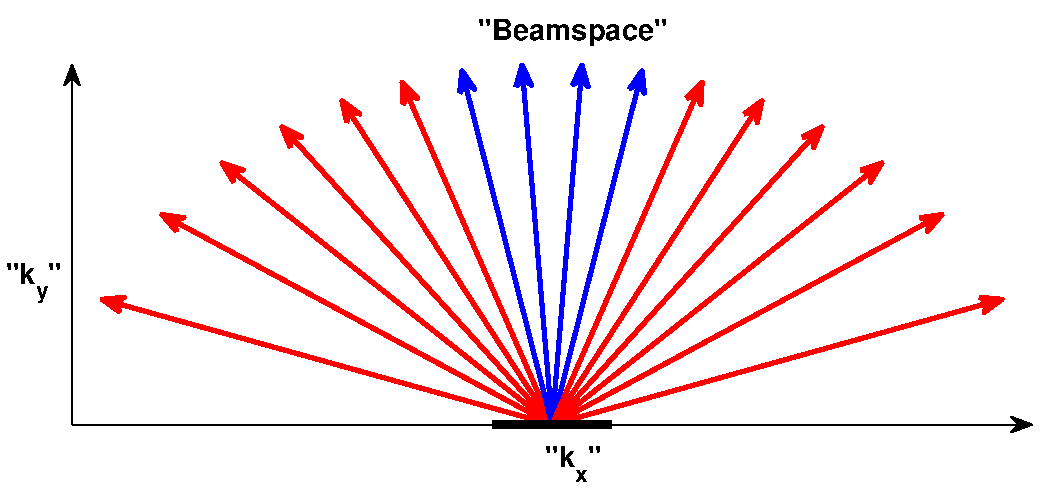
\includegraphics[width=.6\textwidth]{Figs/BeamspaceField}
}

%Carl-Inge Colombo Nilsen, C-I C and Hafizovic, I, \emph{Beamspace
%  Adaptive Beamforming for Ultrasound Imaging}, IEEE Trans. Ultrason. Ferroelectr. Freq. Control, vol. 56, no. 10, Oct 2009.


\section[]{Results}
%\subsection[]{}
\frame{
  \frametitle{Simulated and \\
    experimental results}
  \begin{itemize}
    \rlap{\hspace*{6.5cm}\raisebox{-.5cm}[0pt][0pt]{\mbox{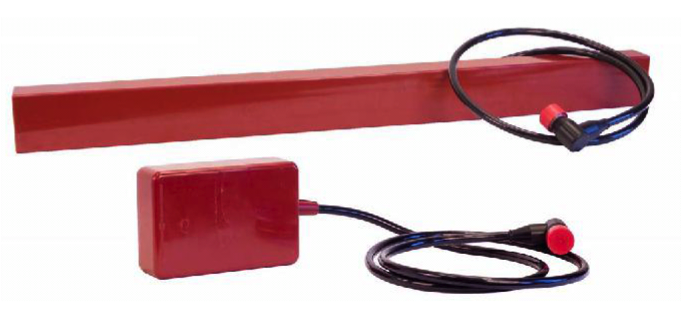
\includegraphics[width=
            .4\textwidth]{Figs/HISAS_1030}}}}
  \item HISAS 1030
    \begin{itemize}
    \item Designed as a High Resolution Interferometric SAS system
    \end{itemize}
  \item Used as a real aperture sonar for sector scan imaging
    \begin{itemize}
    \item Phased-array transmitter-receiver
    \item Transmitter opening angle ~15 deg 
    \item Transmitted pulse: Chirp signal; 85-115 kHz  
    \item  32-element receiver, array length 120 cm
    \item  Receiver element opening angle ~23 deg.
    \item Simulated point reflectors at different depths
    \item Simulated images with speckle, highlight and shadow 
    \end{itemize}
  \item and used as a side-scan sonar on experimental data
  \end{itemize}
}


%\section[]{}
\subsection[]{Simulated point reflectors}
\frame{
  %\frametitle{Point targets}
  \textbf{\Large Simulated point reflectors, one meter apart, located
    at 50 meter and 70 meter}\newline
  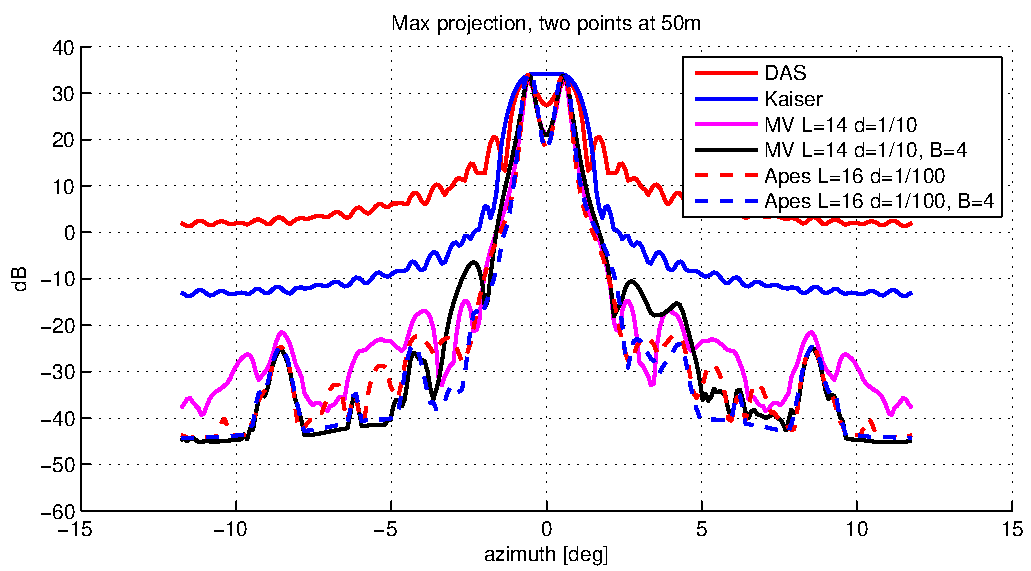
\includegraphics[width=.6\textwidth]{Figs/Pairwise_5_Cuts}\\
  \hspace*{.3\textwidth}
  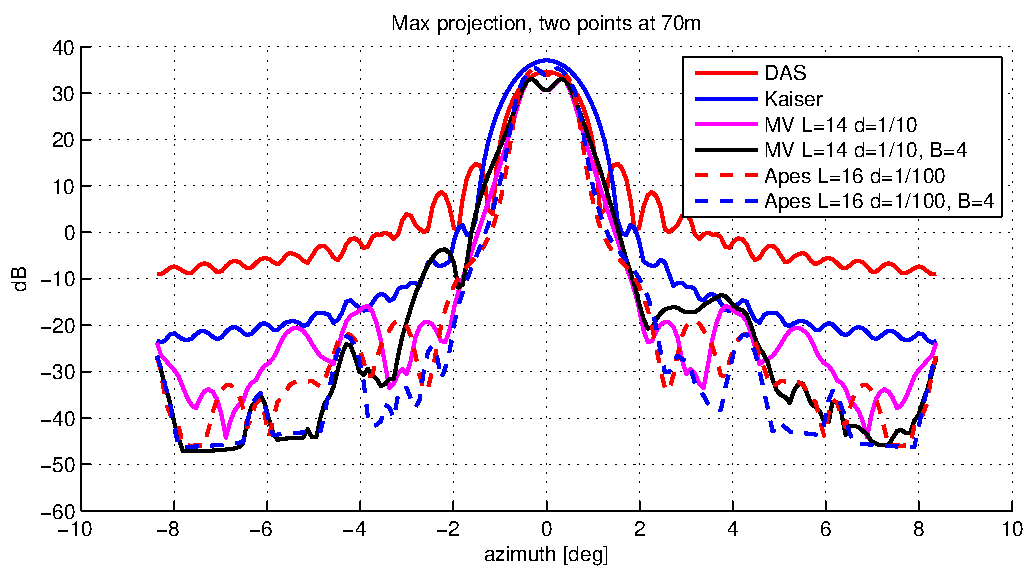
\includegraphics[width=.6\textwidth]{Figs/Pairwise_7_Cuts}
  \vglue -.05\textheight
}


%\section[]{}
\subsection[]{Images of speckle, highlight and shadow}
\frame{
  %  \frametitle{}
  \noindent\textbf{\Large Image of speckle, highlight and
    shadow}\newline
  
  \indent\parbox[t]{.8\textwidth}{\textbf{\large A highlihgt region
      with diameter of 2 meter located at $\approx$41 meters with a
      constant level 15.4 dB above the average speckle region}}\newline
  
  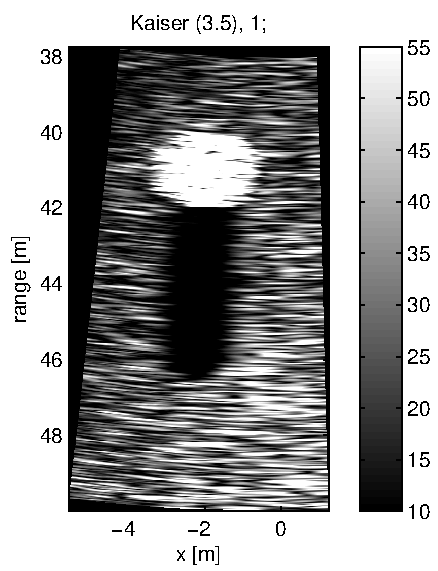
\includegraphics[height=.45\textheight]{Figs/Window_Specle_1_32_1_delta1_0}
  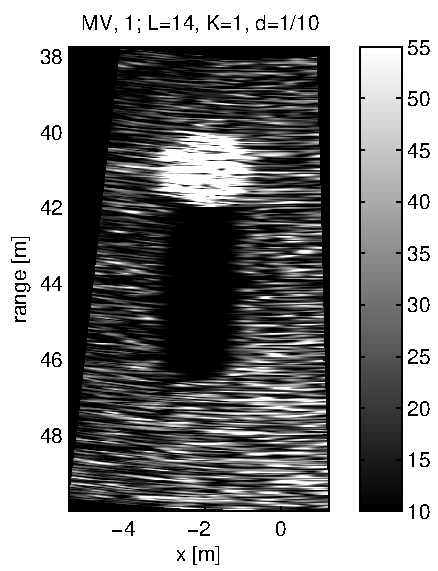
\includegraphics[height=.45\textheight]{Figs/MV_Specle_1_14_1_delta1_10} 
  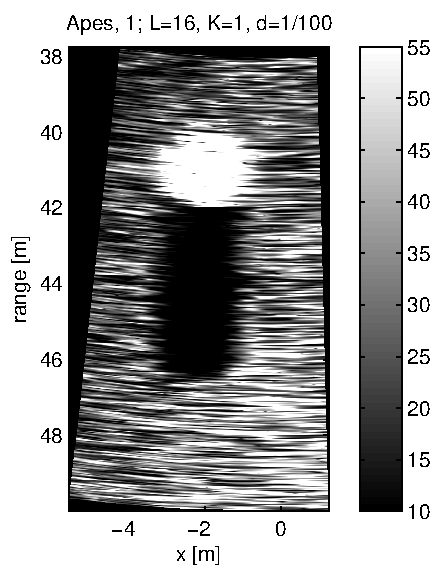
\includegraphics[height=.45\textheight]{Figs/Apes_Specle_1_16_1_delta1_100} 
}

\frame{
    \frametitle{}
  \noindent\textbf{\Large Image of speckle, highlight and
    shadow}\newline
  
  \indent\parbox[t]{.8\textwidth}{\textbf{\large Monte Carlo
      simulation, 100 realizations of speckle. Cut through highlight
      and shadow region.}}\newline
  
  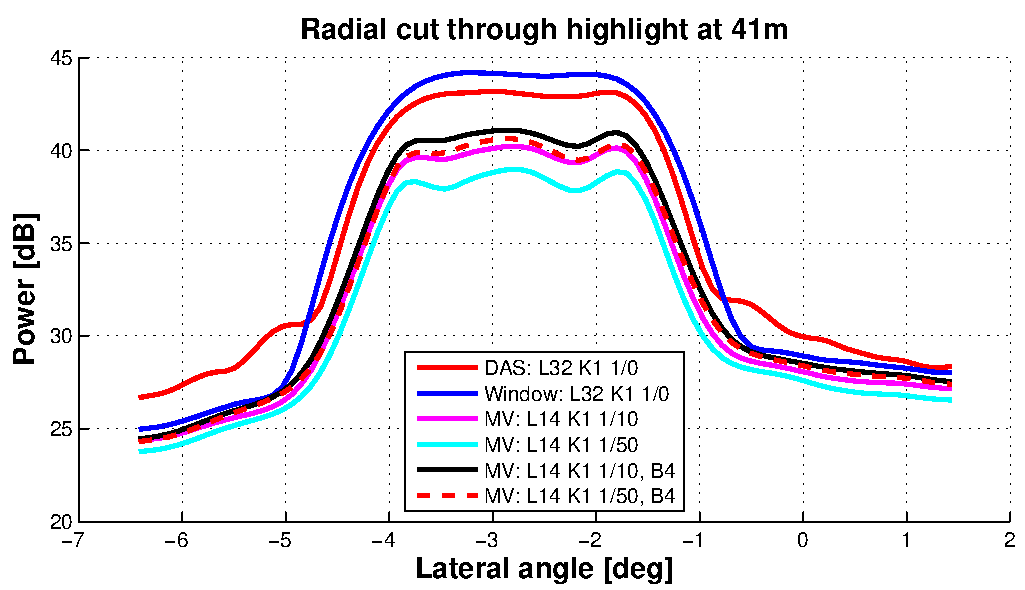
\includegraphics[width=.45\textwidth]{Figs/Real/MVRealizations_Cut41} 
  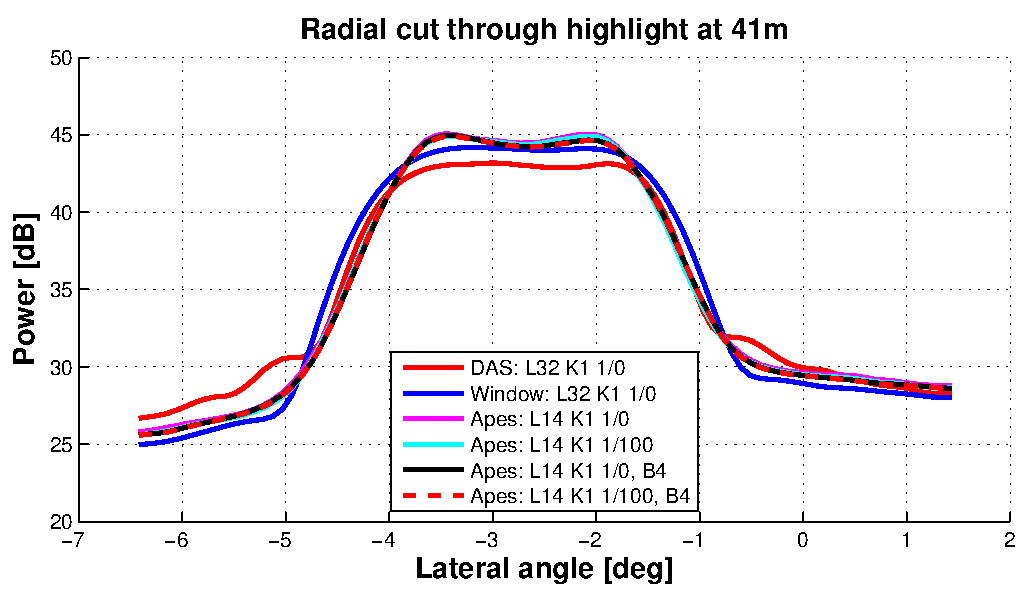
\includegraphics[width=.45\textwidth]{Figs/Real/ApesRealizations_Cut41} \\
  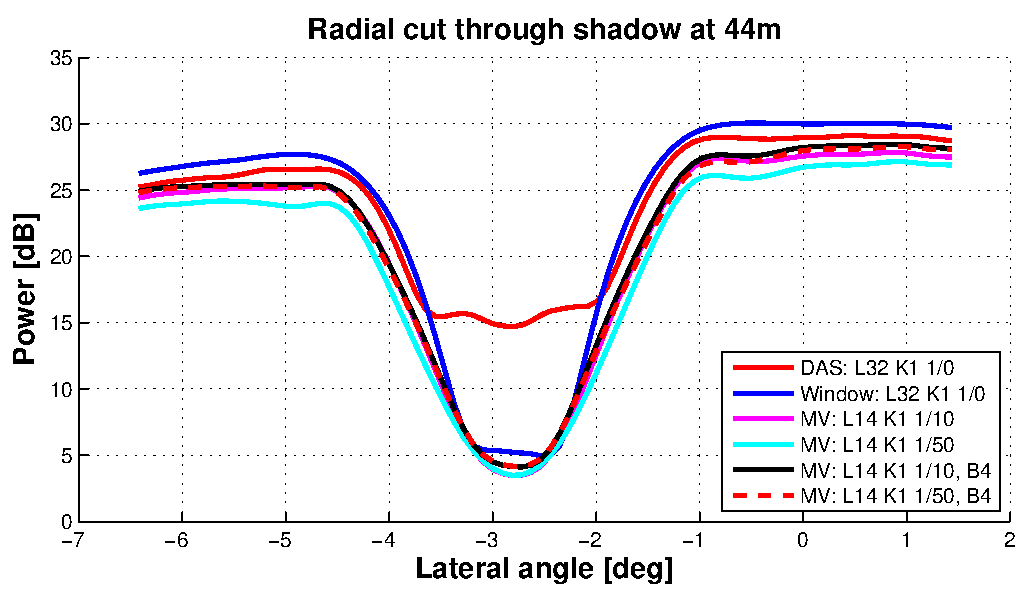
\includegraphics[width=.45\textwidth]{Figs/Real/MVRealizations_Cut44} 
  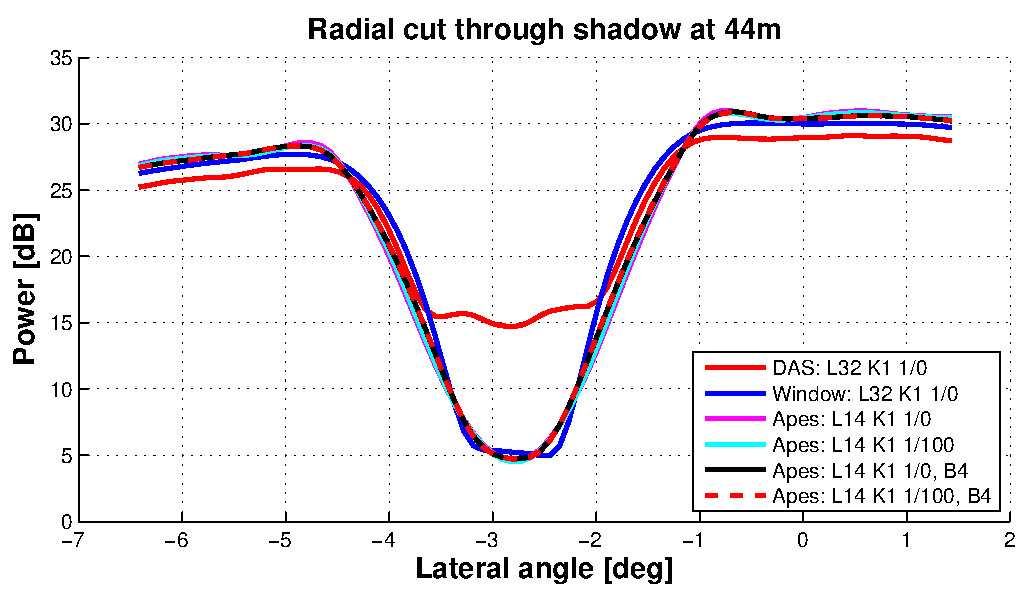
\includegraphics[width=.45\textwidth]{Figs/Real/ApesRealizations_Cut44} 
%  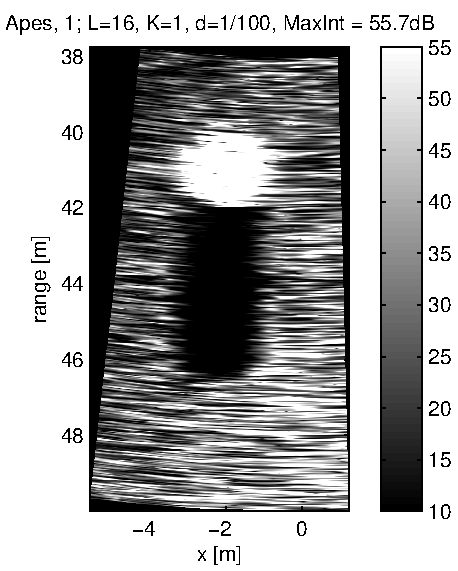
\includegraphics[width=.25\textwidth]{Figs/Real/Apes_Specle_1_16_1_delta1_100} 
}

\subsection[]{Simulated point reflectors}
\frame{
    \frametitle{}
  \noindent\textbf{\Large Image of speckle, highlight and
    shadow}\newline
  \indent\parbox[t]{.8\textwidth}{\textbf{\large Radial through speckle,
      highlight and shadow regions.}}\newline
   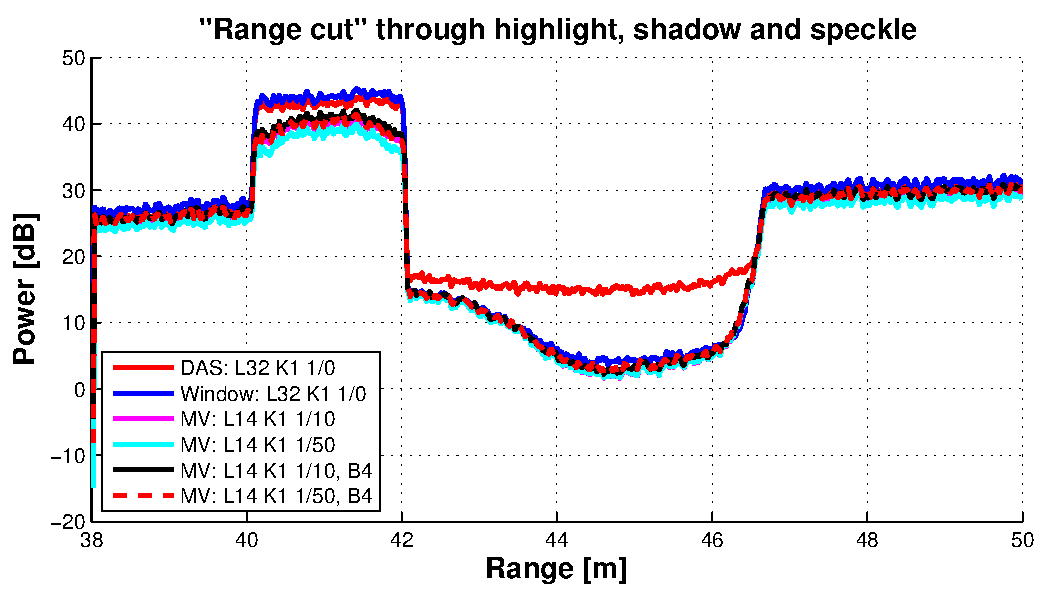
\includegraphics[width=.56\textwidth]{Figs/Real/MVRealizations_RCut}\\
  \hspace*{.3\textwidth}
  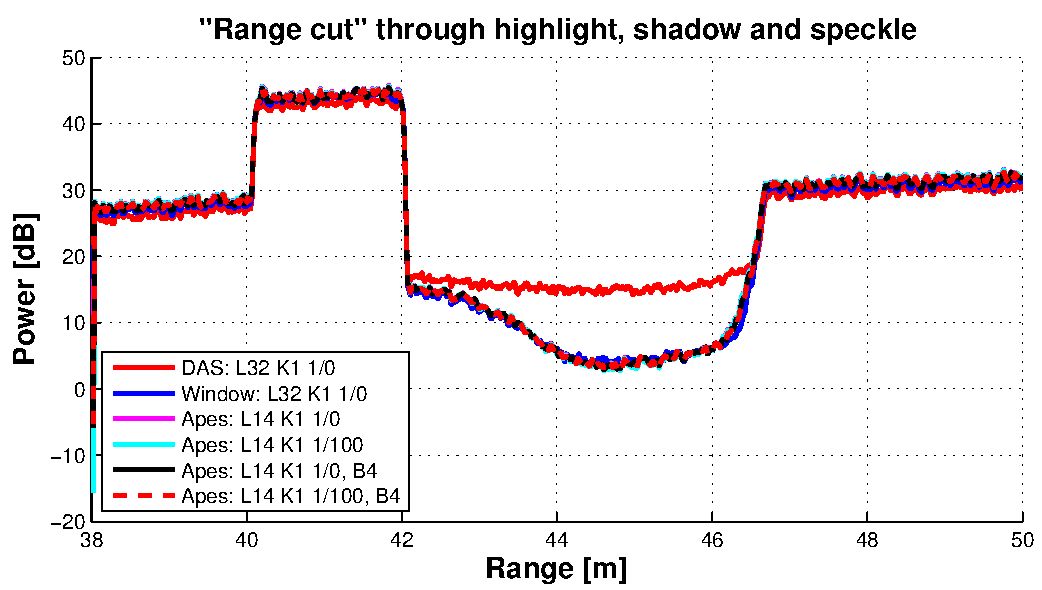
\includegraphics[width=.56\textwidth]{Figs/Real/ApesRealizations_RCut}
%  \vglue -.05\textheight
}



 \subsection[]{Experimental SSS images}
 \begin{frame}
   \frametitle{Experimental SSS images of Holmengraa}
   \indent\parbox[t]{.9\textwidth}{\textbf{\large Distance to the centre of the image is about 95 m. The length of the wreck is about 68m and width about 9m. The wreck of the 1500 dwt oil tanker Holmengraa is lying on a slanted seabed at a depth of 77m.}}\newline
   \centerline{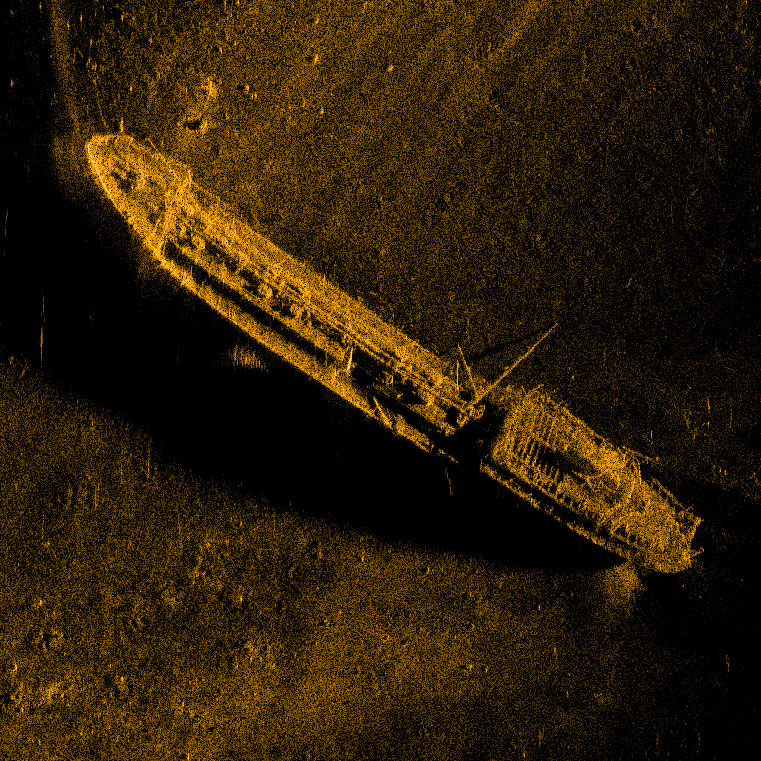
\includegraphics[width=.4\textwidth]{Figs/Holmengraa-761x761}}
 \end{frame}


\frame{
    \frametitle{}
  \noindent\textbf{\Large Experimental SSS images}\newline
    
  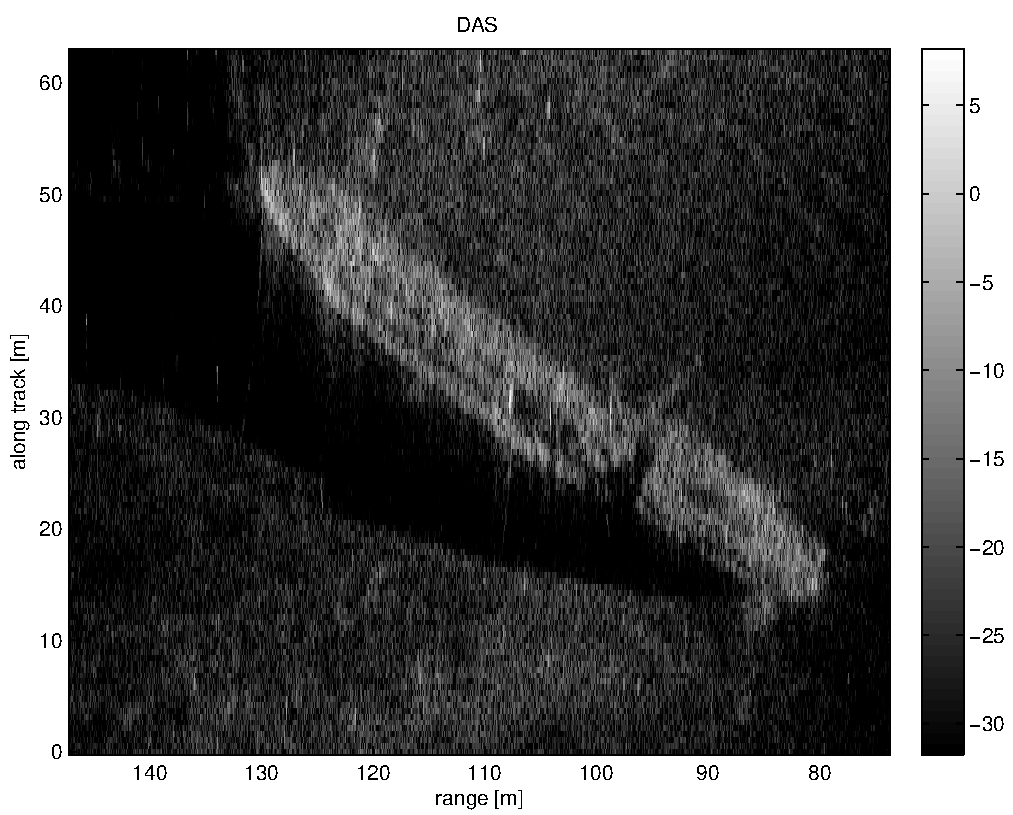
\includegraphics[width=.45\textwidth]{Figs/DAS_Holmengraa_32_1_delta1_0} 
  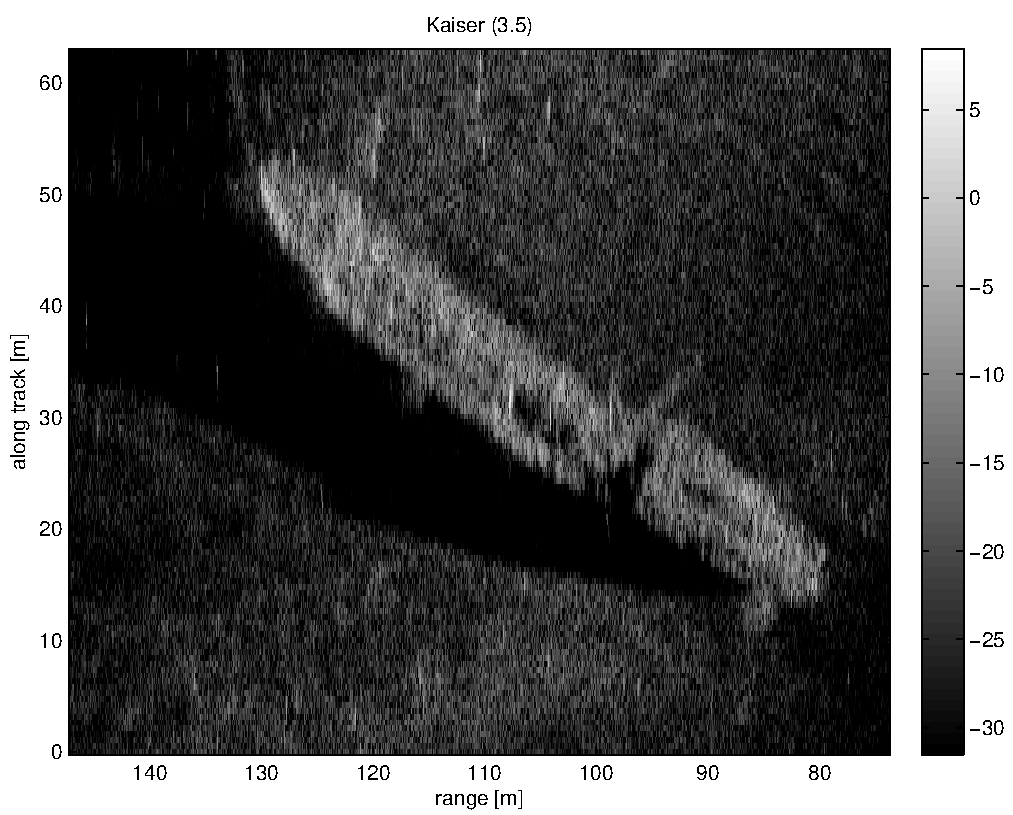
\includegraphics[width=.45\textwidth]{Figs/Window_Holmengraa_32_1_delta1_0} \\
  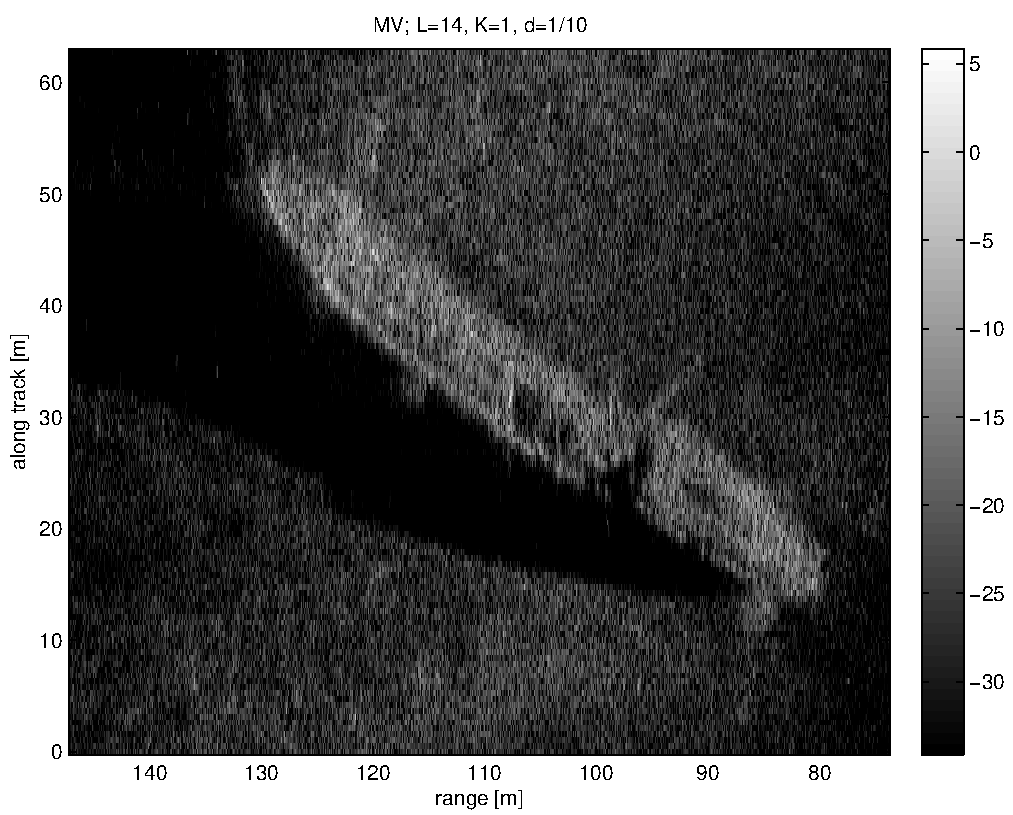
\includegraphics[width=.45\textwidth]{Figs/MV_Holmengraa_14_1_delta1_10} 
  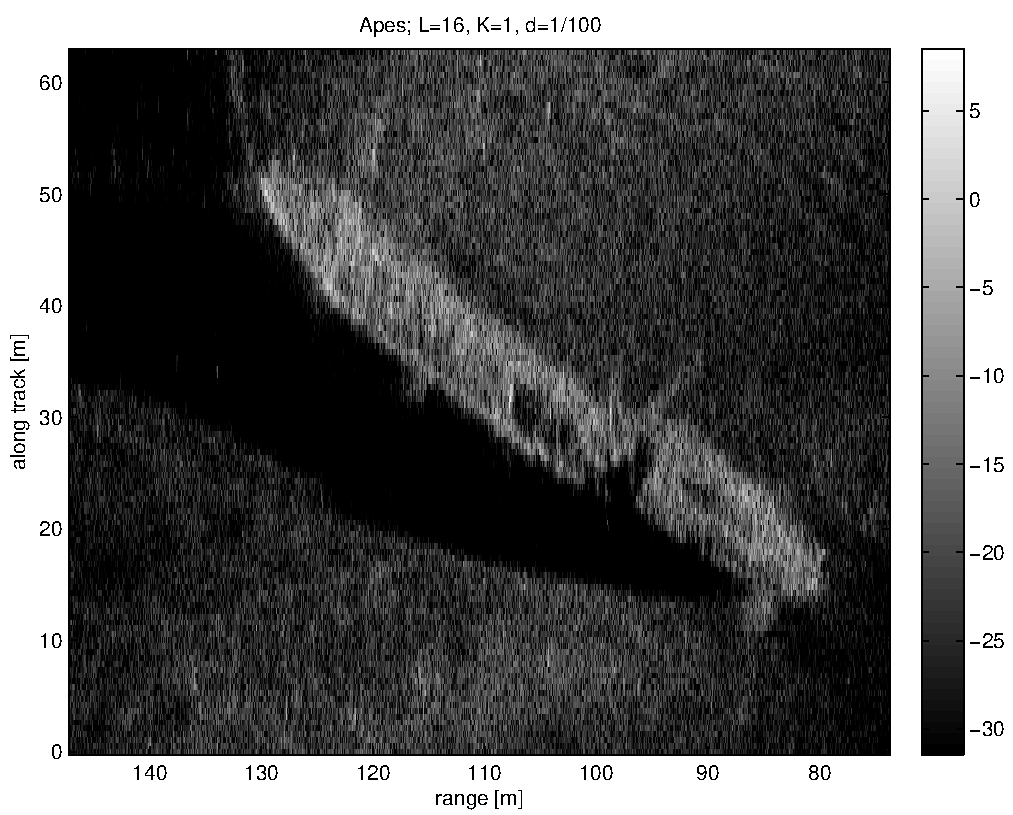
\includegraphics[width=.45\textwidth]{Figs/Apes_Holmengraa_16_1_delta1_100} 
%  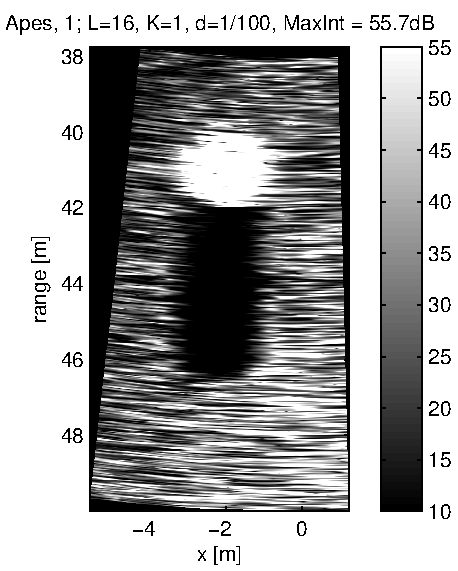
\includegraphics[width=.25\textwidth]{Figs/Real/Apes_Specle_1_16_1_delta1_100} 
}

\frame{
    \frametitle{}
  \noindent\textbf{\Large Experimental SSS images, DAS}\newline
  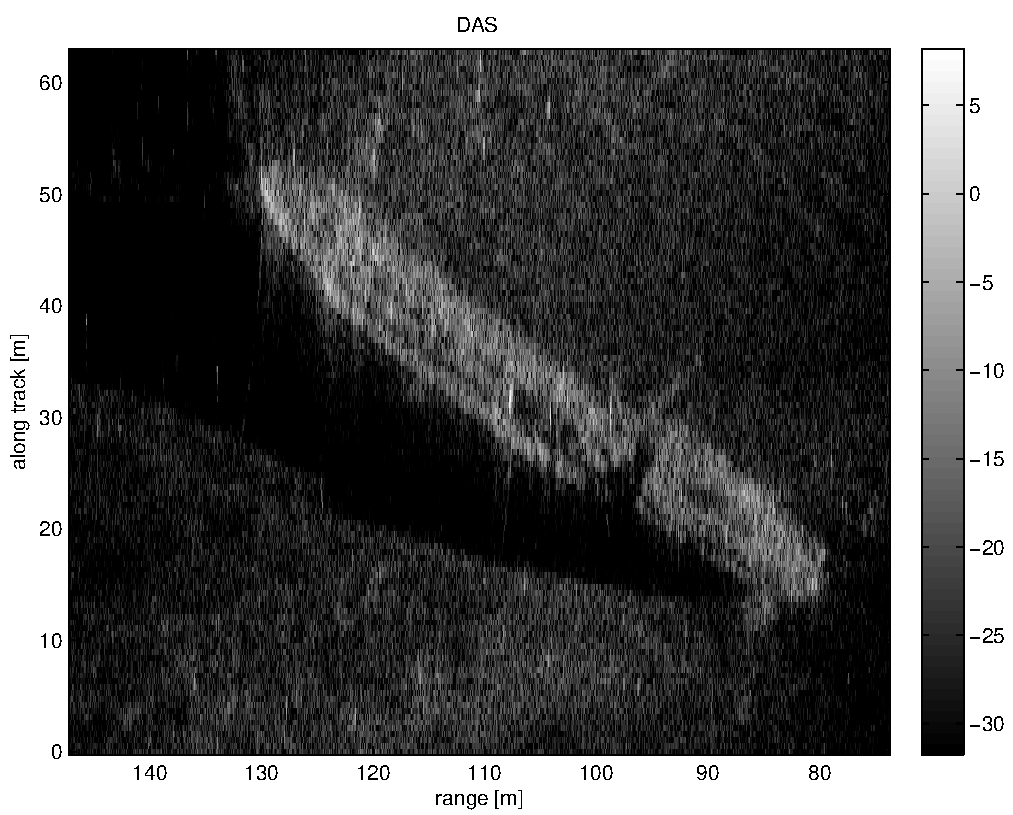
\includegraphics[width=.90\textwidth]{Figs/DAS_Holmengraa_32_1_delta1_0} 
%  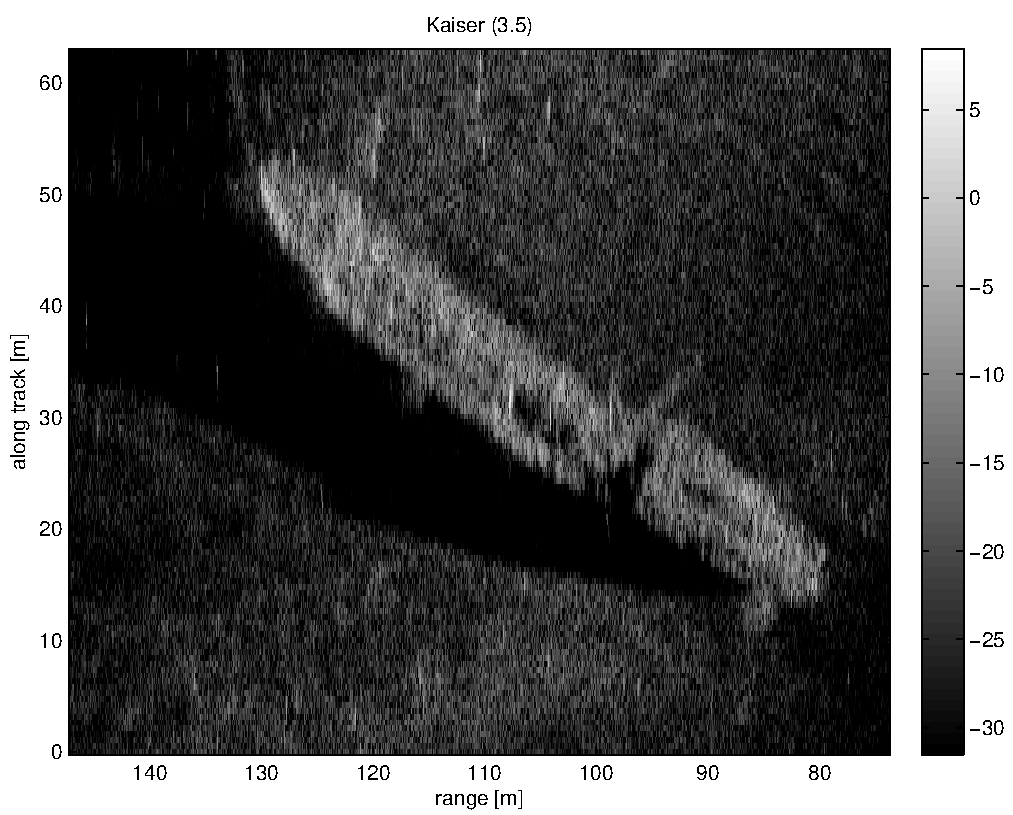
\includegraphics[width=.45\textwidth]{Figs/Window_Holmengraa_32_1_delta1_0} \\
%  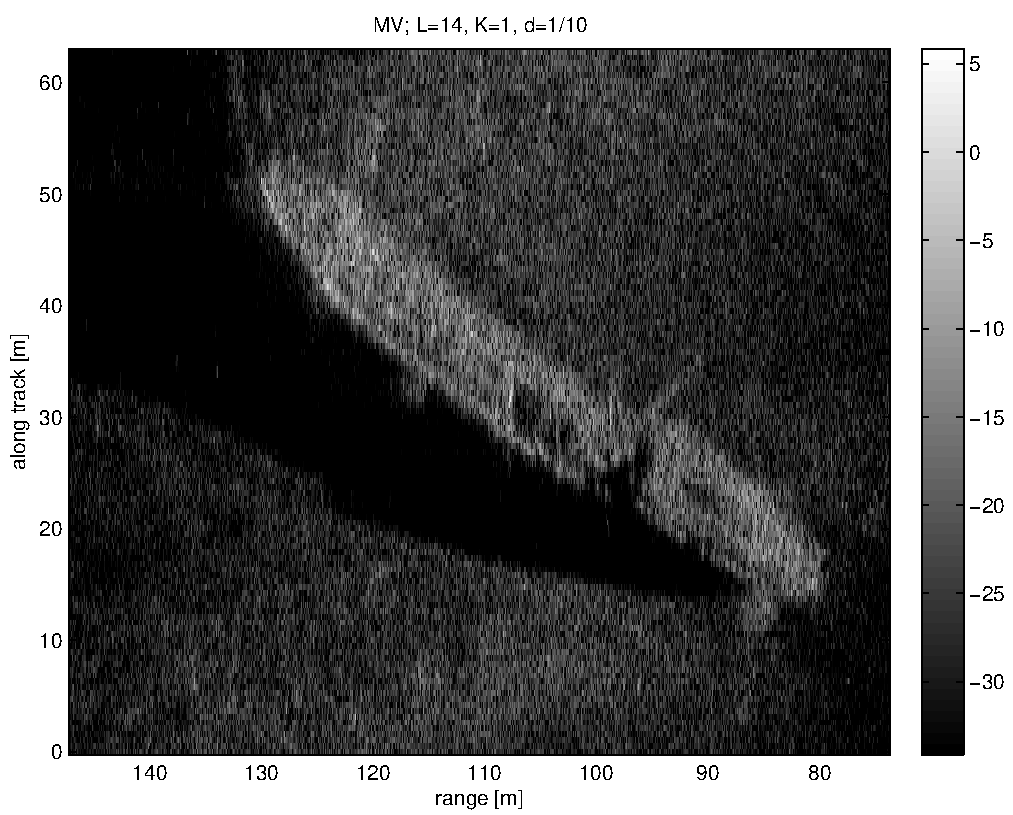
\includegraphics[width=.45\textwidth]{Figs/MV_Holmengraa_14_1_delta1_10} 
%  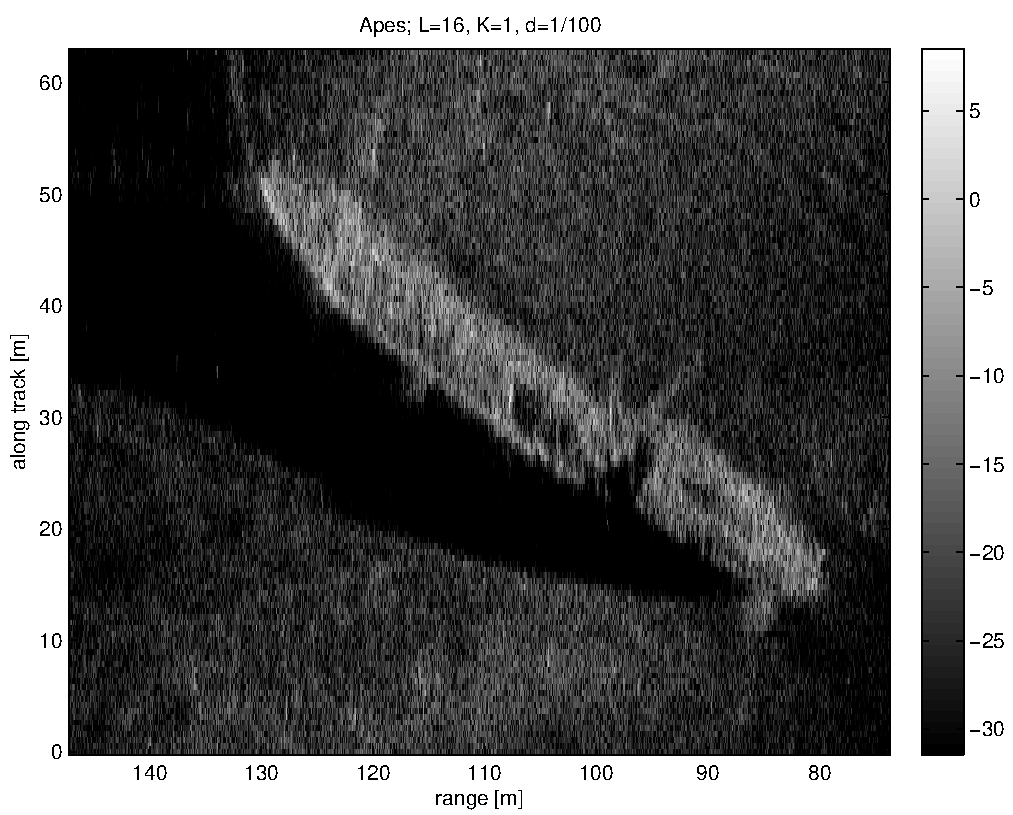
\includegraphics[width=.45\textwidth]{Figs/Apes_Holmengraa_16_1_delta1_100} 
}


\frame{
    \frametitle{}
  \noindent\textbf{\Large Experimental SSS images, Kaiser 3.5}\newline
%  \includegraphics[width=.90\textwidth]{Figs/Das_Holmengraa_32_1_delta1_0} 
  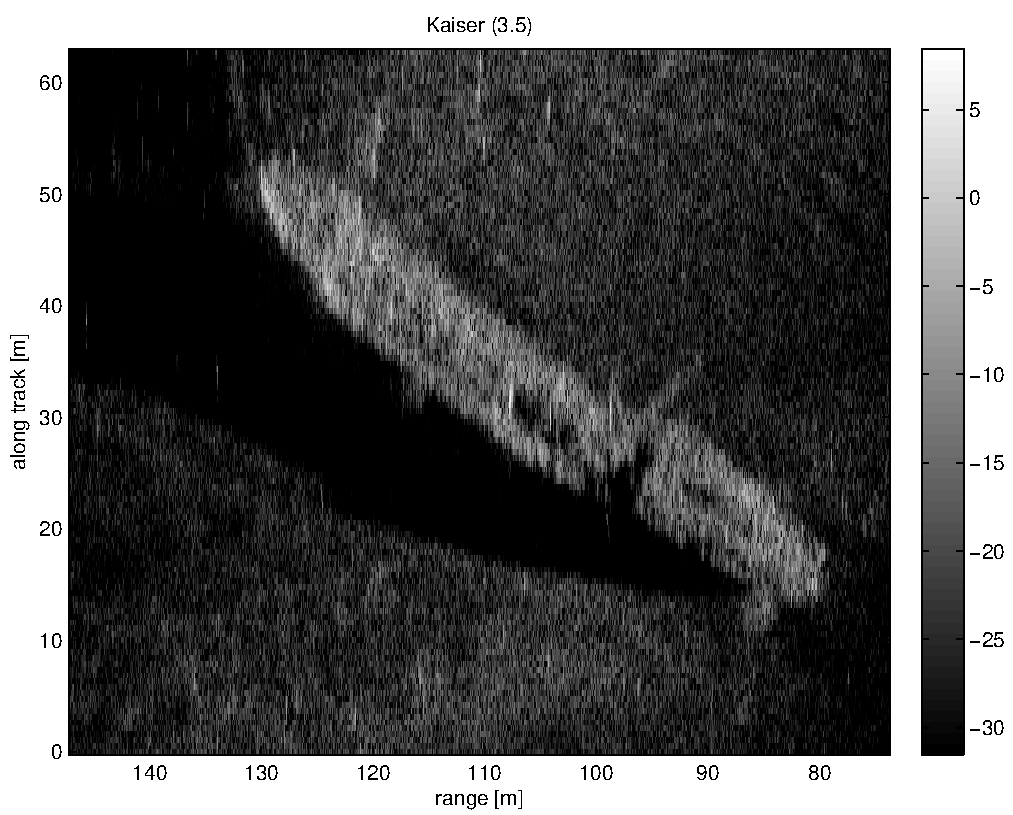
\includegraphics[width=.90\textwidth]{Figs/Window_Holmengraa_32_1_delta1_0} \\
%  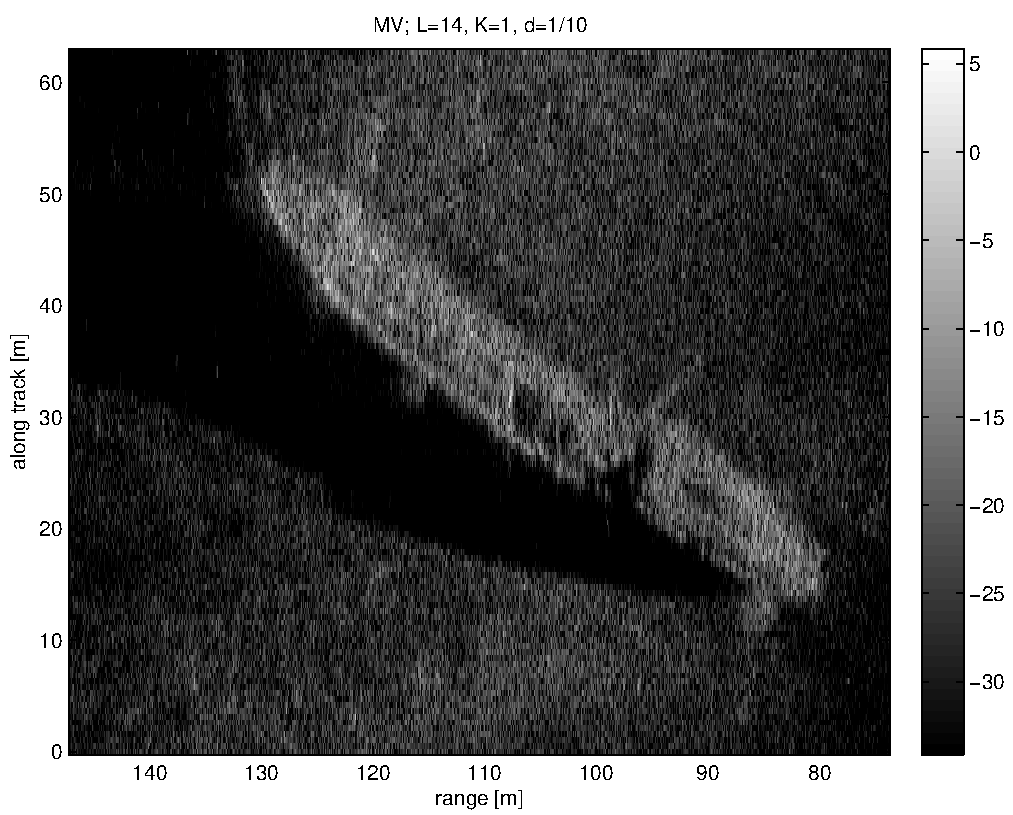
\includegraphics[width=.45\textwidth]{Figs/MV_Holmengraa_14_1_delta1_10} 
%  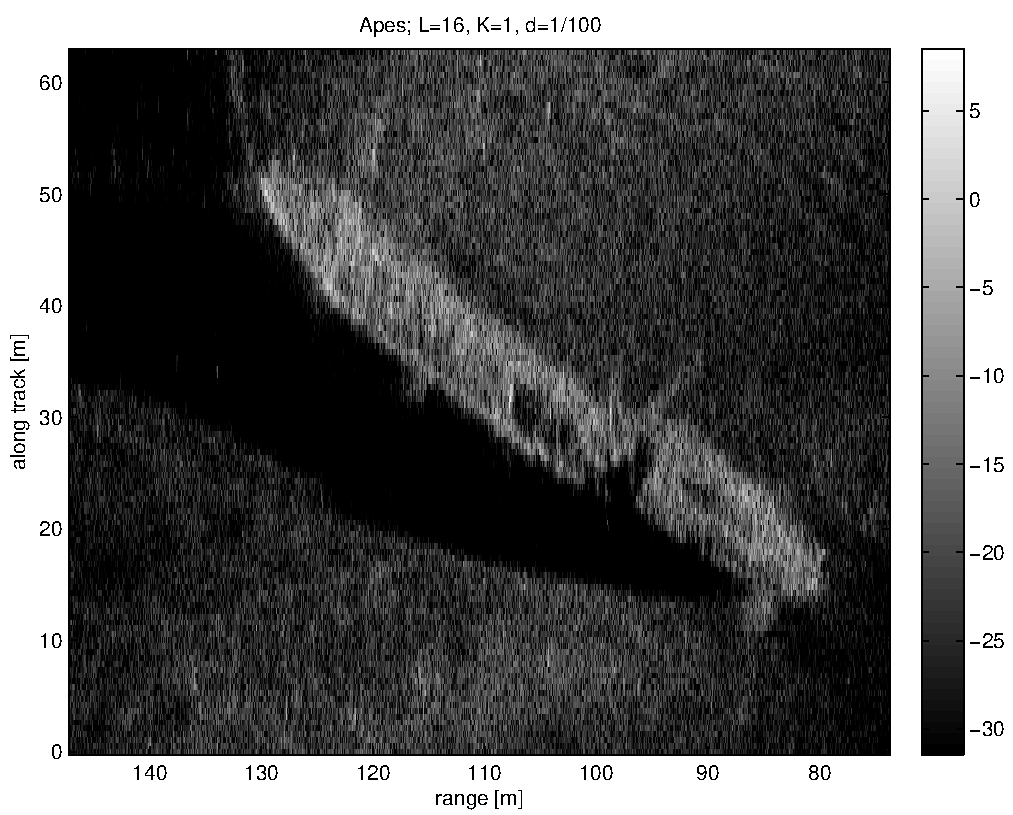
\includegraphics[width=.45\textwidth]{Figs/Apes_Holmengraa_16_1_delta1_100} 
}


\frame{
    \frametitle{}
  \noindent\textbf{\Large Experimental SSS images, MV}\newline
%  \includegraphics[width=.90\textwidth]{Figs/Das_Holmengraa_32_1_delta1_0} 
%  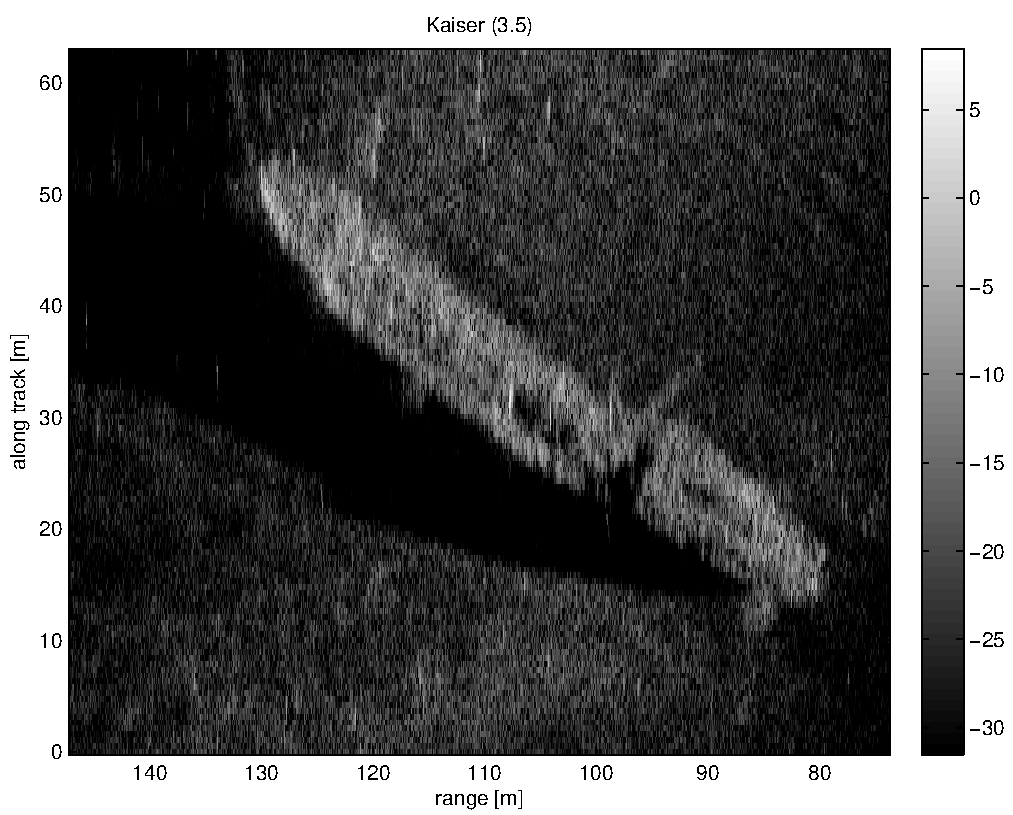
\includegraphics[width=.45\textwidth]{Figs/Window_Holmengraa_32_1_delta1_0} \\
  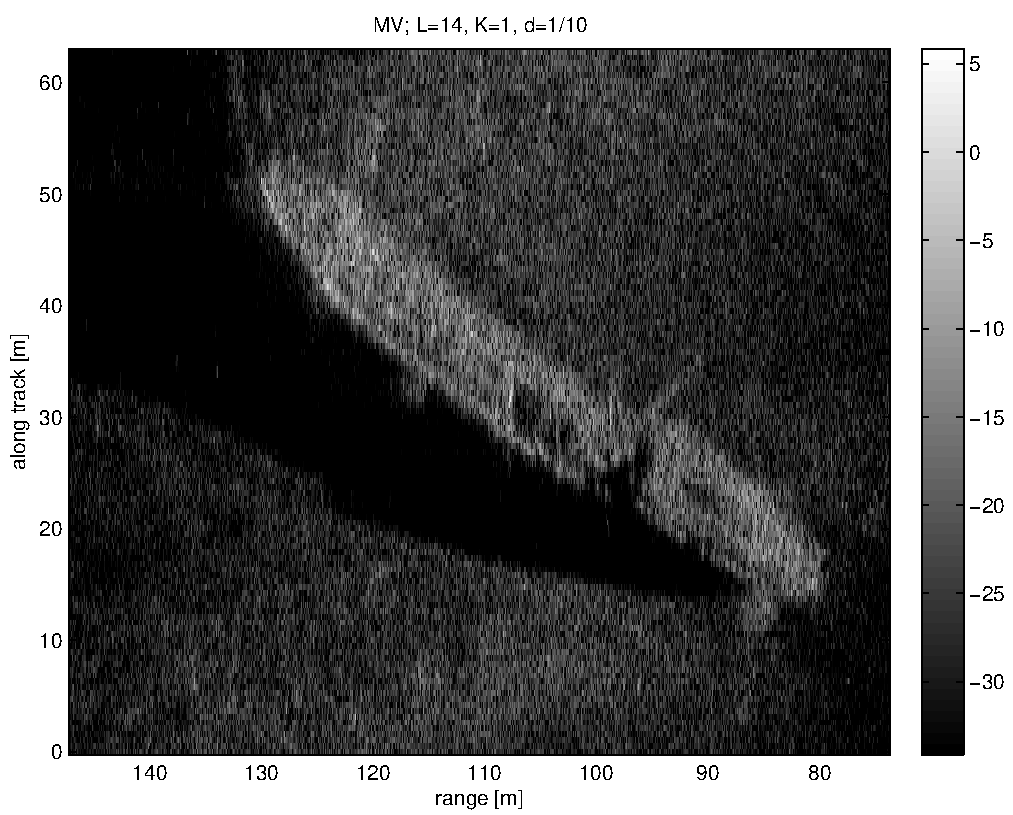
\includegraphics[width=.90\textwidth]{Figs/MV_Holmengraa_14_1_delta1_10} 
%  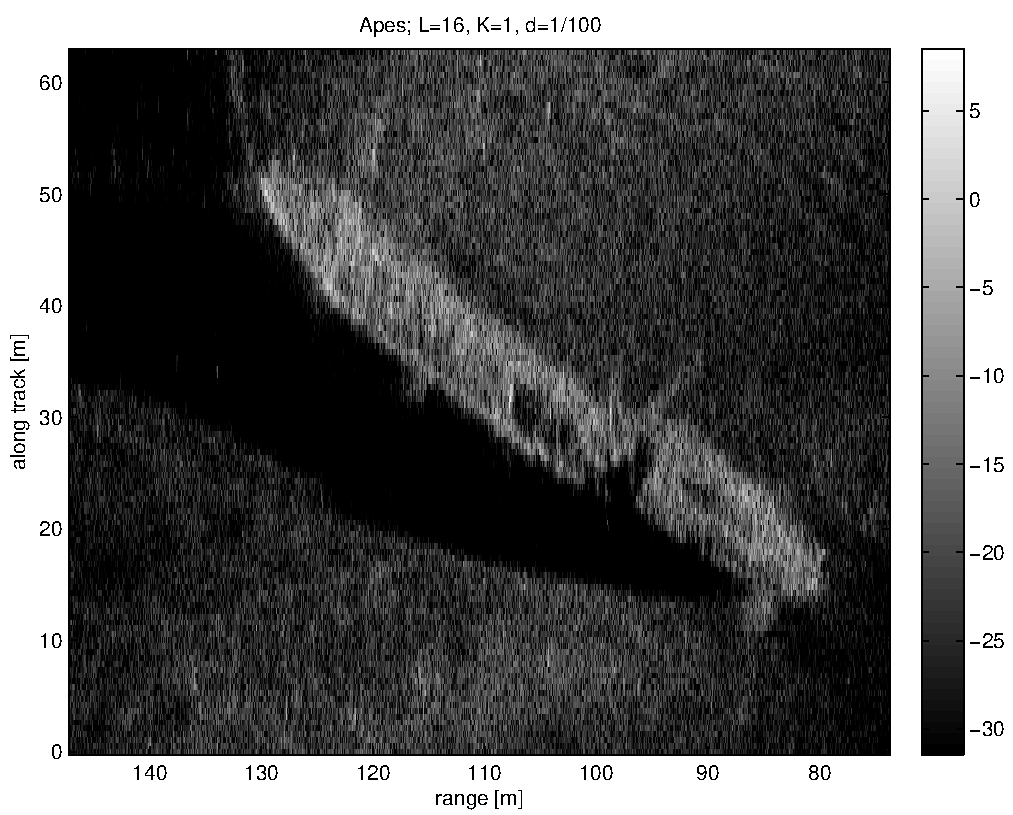
\includegraphics[width=.45\textwidth]{Figs/Apes_Holmengraa_16_1_delta1_100} 
}

\frame{
    \frametitle{}
  \noindent\textbf{\Large Experimental SSS images, MV, Bdim=4}\newline
%  \includegraphics[width=.90\textwidth]{Figs/Das_Holmengraa_32_1_delta1_0} 
%  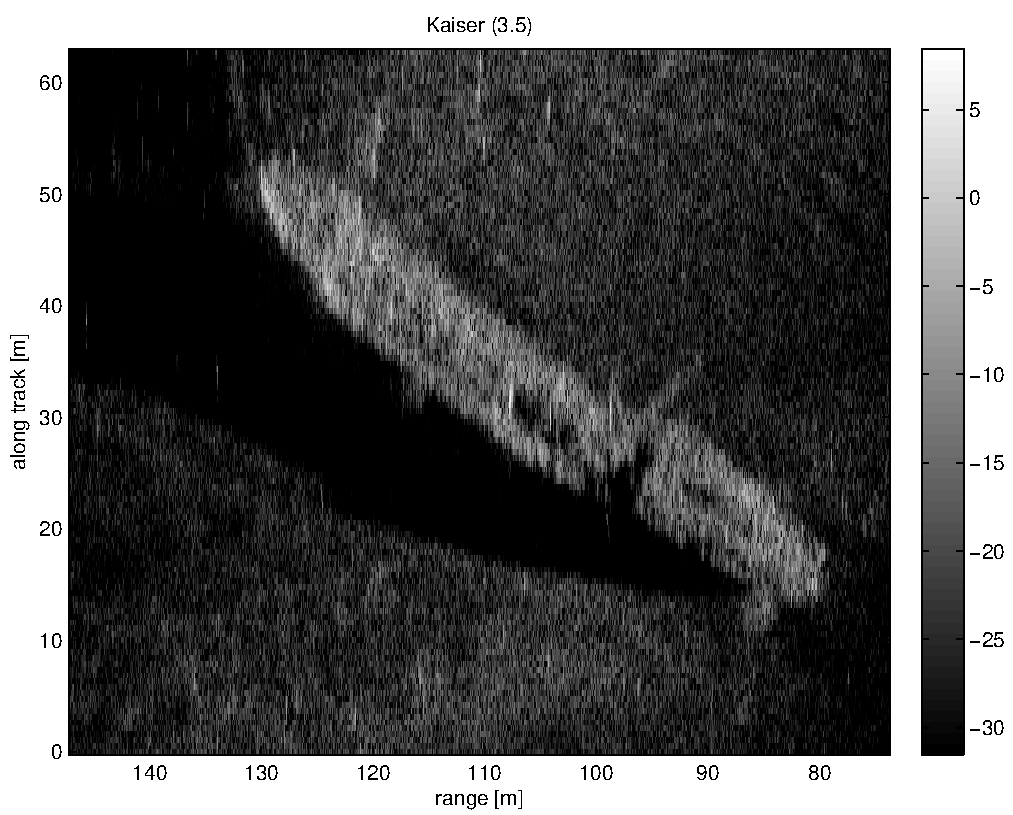
\includegraphics[width=.45\textwidth]{Figs/Window_Holmengraa_32_1_delta1_0} \\
  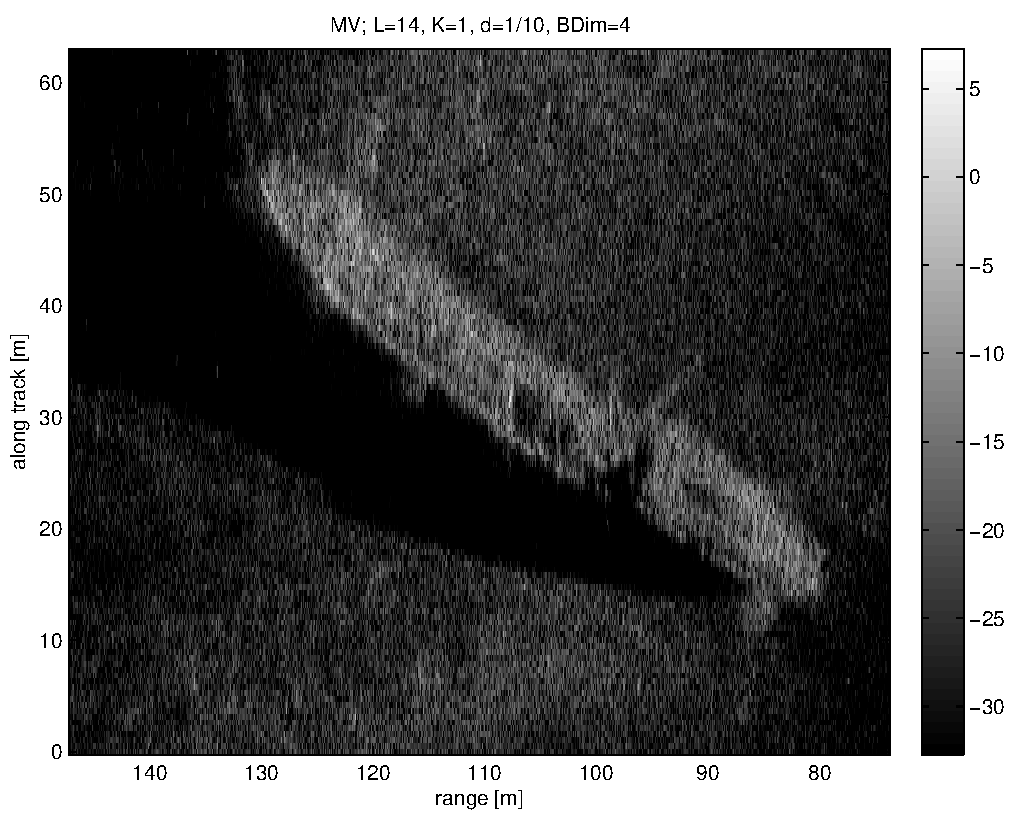
\includegraphics[width=.90\textwidth]{Figs/MV_Holmengraa_14_1_delta1_10_SubSp_4} 
%  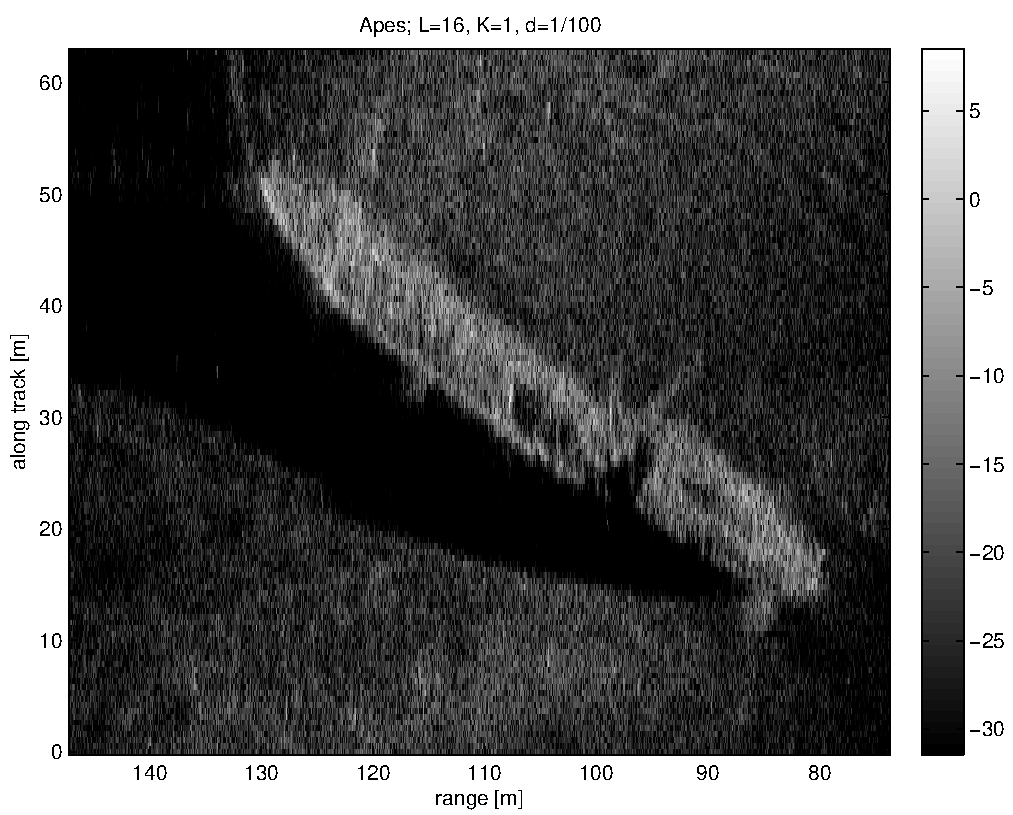
\includegraphics[width=.45\textwidth]{Figs/Apes_Holmengraa_16_1_delta1_100} 
}


\frame{
    \frametitle{}
  \noindent\textbf{\Large Experimental SSS images, Apes}\newline
%  \includegraphics[width=.90\textwidth]{Figs/Das_Holmengraa_32_1_delta1_0} 
%  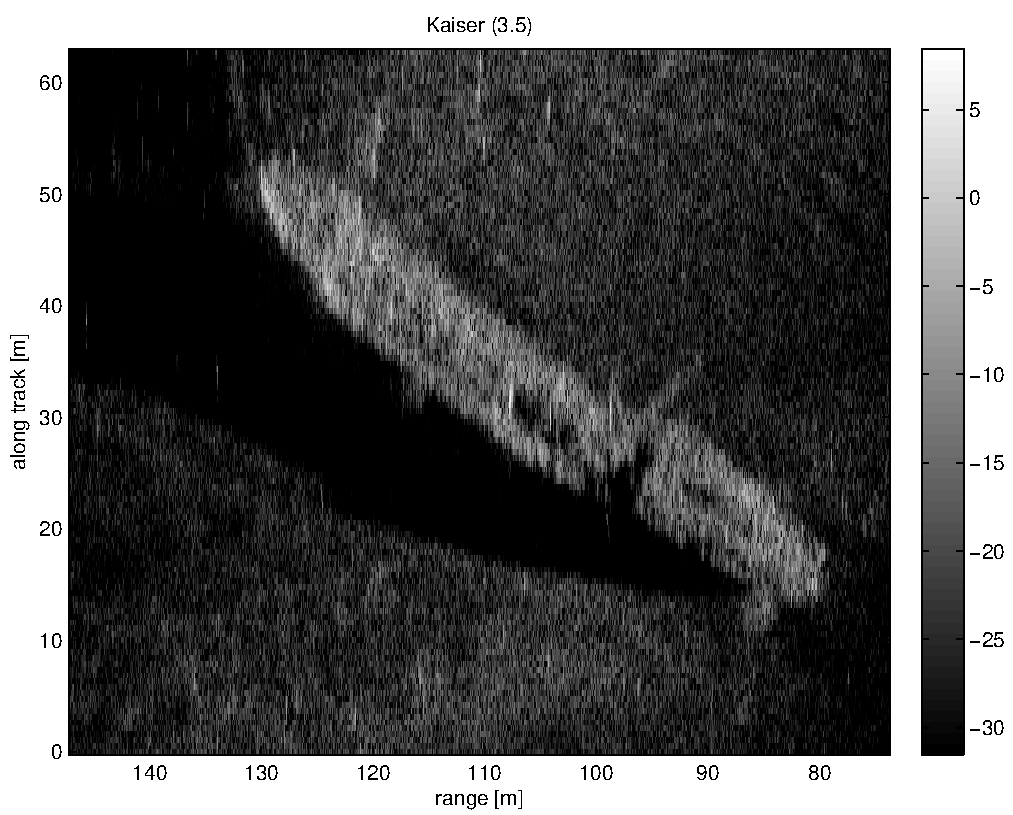
\includegraphics[width=.45\textwidth]{Figs/Window_Holmengraa_32_1_delta1_0} \\
%  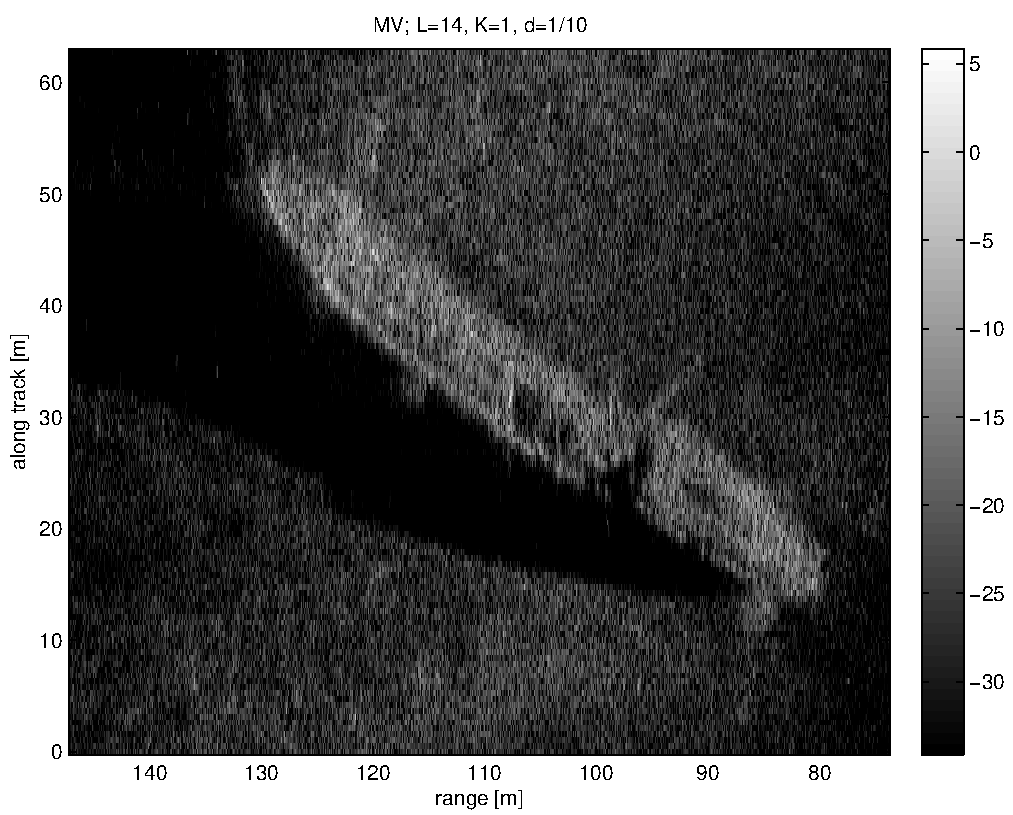
\includegraphics[width=.45\textwidth]{Figs/MV_Holmengraa_14_1_delta1_10} 
  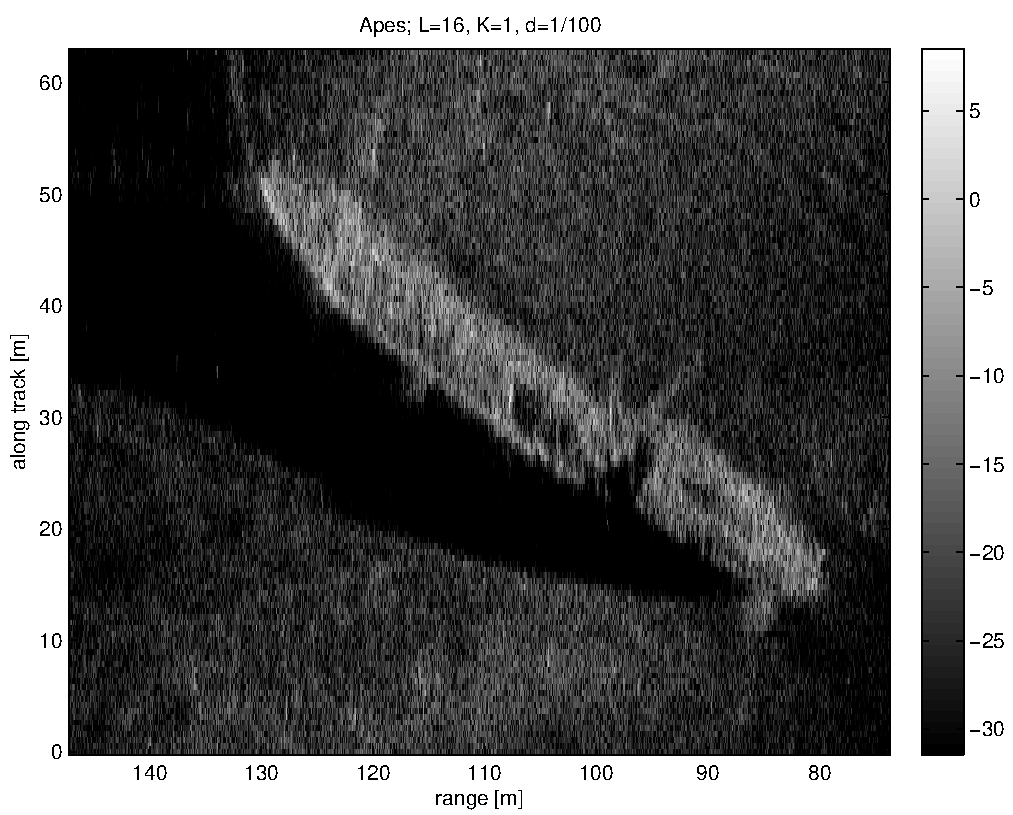
\includegraphics[width=.90\textwidth]{Figs/Apes_Holmengraa_16_1_delta1_100} 
}

\frame{
    \frametitle{}
  \noindent\textbf{\Large Experimental SSS images, Apes, Bdim=4}\newline
%  \includegraphics[width=.90\textwidth]{Figs/Das_Holmengraa_32_1_delta1_0} 
%  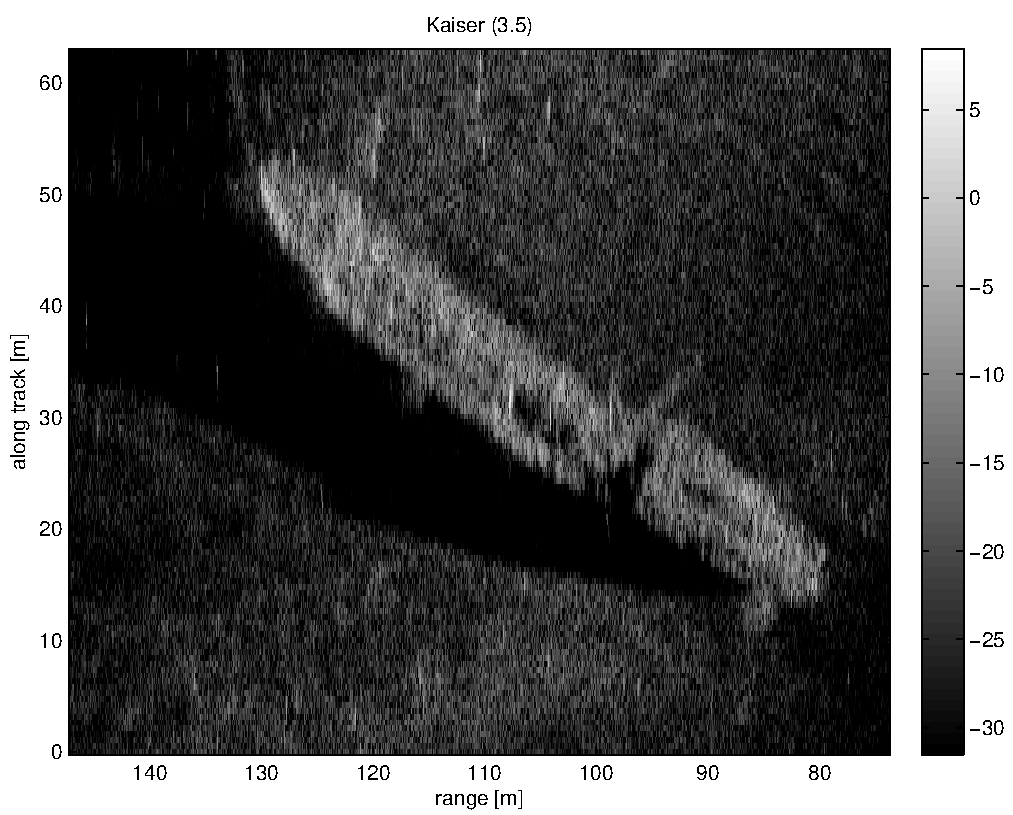
\includegraphics[width=.45\textwidth]{Figs/Window_Holmengraa_32_1_delta1_0} \\
%  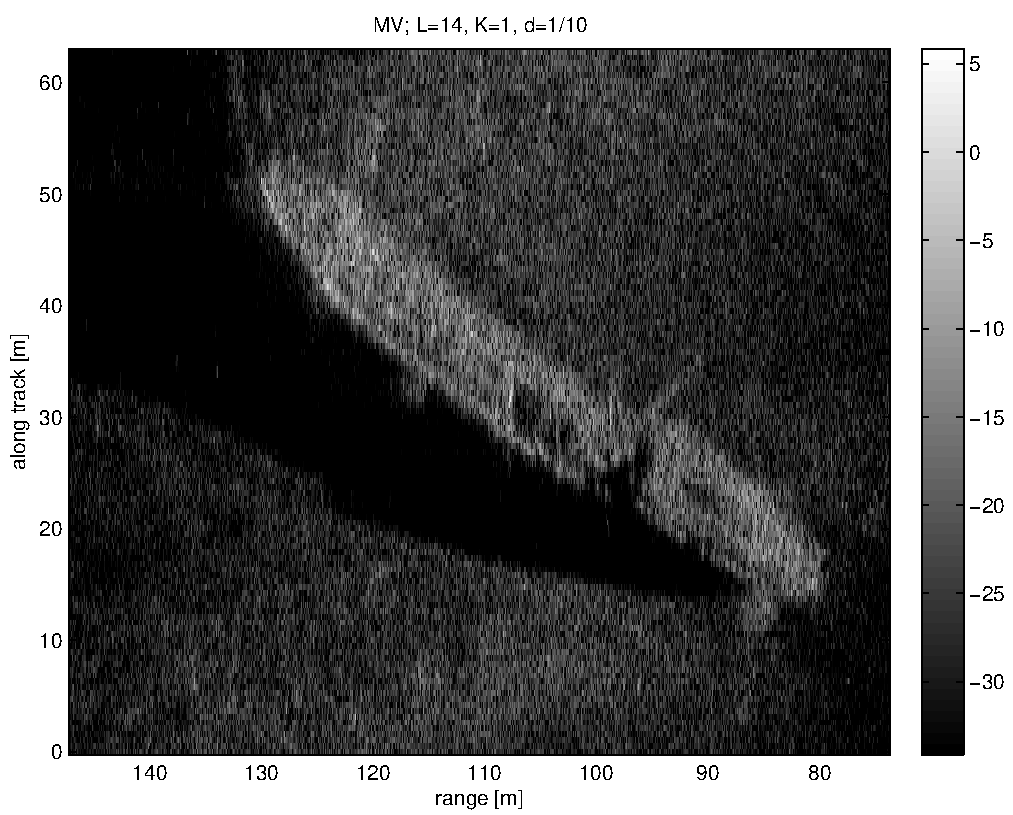
\includegraphics[width=.45\textwidth]{Figs/MV_Holmengraa_14_1_delta1_10} 
  \includegraphics[width=.90\textwidth]{Figs/Apes_Holmengraa_16_1_delta1_100_SubSp_4} 
}

\frame{
    \frametitle{}
  \noindent\textbf{\Large Experimental SSS images, Kaiser 3.5}\newline
%  \includegraphics[width=.90\textwidth]{Figs/Das_Holmengraa_32_1_delta1_0} 
  \includegraphics[width=.90\textwidth]{Figs/Window_Holmengraa_32_1_delta1_0} \\
%  \includegraphics[width=.45\textwidth]{Figs/MV_Holmengraa_14_1_delta1_10} 
%  \includegraphics[width=.45\textwidth]{Figs/Apes_Holmengraa_16_1_delta1_100} 
}

 \section[]{Conclusion}
 \begin{frame}
 \frametitle{Conclusion}
   \begin{itemize}
   \item Presented simulated and experimental images from conventional
     and adaptive beamformers
   \item Showed that adaptive BF produces
     \begin{itemize}
     \item edge responses that are better or comparable with
       conventional BF (with or without weighting/tapering)
     \item a sidelobe level or filling of shadow regions comparable to
       a Kaiser weighted DAS beamformer.
     \end{itemize}
   \item Showed that beamspace processing does reduce computational
     complexity without degrading image quality.
   \end{itemize}
 \end{frame}



%%%%%%%%%%%%%%%%%%%%%%%%%%%%%%%%%%%%%%%%%%%%%%%%%%%%%%%%%%%%%%%%%%%%%%
%%
%% Slutt ...
%%

% \subsection[]{}
% \begin{frame}
% \frametitle{}
%   \begin{itemize}
%   \item 
%   \end{itemize}
% \end{frame}

% \subsection[]{}
% \begin{frame}
% \frametitle{}
%   \begin{itemize}
%   \item 
%   \end{itemize}
% \end{frame}

% \subsection[]{}
% \begin{frame}
% \frametitle{}
%   \begin{itemize}
%   \item 
%   \end{itemize}
% \end{frame}




\end{document}




% \section{}
% \subsection{}
% \begin{frame}
% \frametitle{}
%   \begin{itemize}
%   \item 
%   \end{itemize}
% \end{frame}
% \note{\null{}}

% \section{}
% \subsection{}
% \begin{frame}
% \frametitle{}
%   \begin{itemize}
%   \item 
%   \end{itemize}
% \end{frame}
% \note{\null{}}

% \section{}
% \subsection{}
% \begin{frame}
% \frametitle{}
%   \begin{itemize}
%   \item 
%   \end{itemize}
% \end{frame}
% \note{\null{}}

% \section{}
% \subsection{}
% \begin{frame}
% \frametitle{}
%   \begin{itemize}
%   \item 
%   \end{itemize}
% \end{frame}
% \note{\null{}}

% \section{}
% \subsection{}
% \begin{frame}
% \frametitle{}
%   \begin{itemize}
%   \item 
%   \end{itemize}
% \end{frame}
% \note{\null{}}

% \section{}
% \subsection{}
% \begin{frame}
% \frametitle{}
%   \begin{itemize}
%   \item 
%   \end{itemize}
% \end{frame}
% \note{\null{}}

% \section{}
% \subsection{}
% \begin{frame}
% \frametitle{}
%   \begin{itemize}
%   \item 
%   \end{itemize}
% \end{frame}
% \note{\null{}}

%%%%%%%%%%%%%%%%%%%%%%%%%%%%%%%%%%%%%%%%%%%%%%%%%%%%%%%%%%%%%%%%%%%%%%
%%
%% Slutt ...
%%

% \subsection[]{}
% \begin{frame}
% \frametitle{}
%   \begin{itemize}
%   \item 
%   \end{itemize}
% \end{frame}
% \note{\null{}}

% \subsection[]{}
% \begin{frame}
% \frametitle{}
%   \begin{itemize}
%   \item 
%   \end{itemize}
% \end{frame}
% \note{\null{}}

% \subsection[]{}
% \begin{frame}
% \frametitle{}
%   \begin{itemize}
%   \item 
%   \end{itemize}
% \end{frame}
% \note{\null{}}

Made using the HUGIN 1000 AUV. Distance to the centre of the image is about 95 m. The length of the wreck is about 68m and width about 9m. The wreck of the 1500 dwt oil tanker Holmengraa is lying on a slanted seabed at a depth of 77m.
